\documentclass{beamer}

\usepackage[utf8x]{inputenc}
\usepackage{graphicx}
\usepackage{amsthm,amssymb,amsbsy,amsmath,amsfonts,amssymb,amscd}
\usepackage{dsfont}
\usepackage{array}
\newcolumntype{N}{@{}m{2pt}@{}}
\usepackage{tikz}
%\usetikzlibrary{arrows}
%\tikzstyle{block}=[draw opacity=0.7,line width=1.4cm]

\useoutertheme[subsection=false]{miniframes}
\usepackage{lmodern}

\setbeamercolor{author in head/foot}{fg=gray,bg=white}
\setbeamercolor{title in head/foot}{fg=gray,bg=white}
\setbeamercolor{page number in head/foot}{fg=gray,bg=white}
\setbeamercolor{section in head/foot}{bg=black,fg=gray}
\setbeamercolor{subsection in head/foot}{bg=black,fg=gray}

%%%%%%%%%%%%%%%%%%%%%%%%
% GENERAL BEAMER STYLE :

\setbeamertemplate{footline}{
  \hbox{%
    \begin{beamercolorbox}[wd=.2\paperwidth,ht=2ex,dp=1ex,left]{author in head/foot}%
      \hskip1em\usebeamerfont{author in head/foot}\insertshortauthor
    \end{beamercolorbox}%
    \begin{beamercolorbox}[wd=.7\paperwidth,ht=2ex,dp=1ex,center]{title in head/foot}%
      \usebeamerfont{title in head/foot}\insertshorttitle
    \end{beamercolorbox}%
    \begin{beamercolorbox}[wd=.1\paperwidth,ht=2ex,dp=1ex,right]{page number in head/foot}%
      \usebeamerfont{page number in head/foot}\insertframenumber{} / \inserttotalframenumber
      \kern1em 
    \end{beamercolorbox}
  }
}

\setbeamercolor{alerted text}{fg=red!80!black}
\setbeamercolor{itemize/enumerate subbody}{fg=gray!70!black}
\setbeamertemplate{itemize item}[square]
\setbeamertemplate{itemize subitem}[triangle]%{{\textendash}}
\setbeamerfont{itemize/enumerate subbody}{size=\footnotesize}
\setbeamerfont{itemize/enumerate subitem}{size=\footnotesize}

\setbeamertemplate{navigation symbols}{}

\AtBeginSection{
\begin{frame}
    \begin{centering}
    \begin{beamercolorbox}[sep=12pt,center]{part title}
    \usebeamerfont{section title}\insertsection\par
    \end{beamercolorbox}
    \end{centering}
\end{frame}
}

 

\DeclareMathOperator*{\Var}{var}
\DeclareMathOperator*{\E}{E}
\DeclareMathOperator*{\Cov}{cov}
\newcommand\PR[1]{\mathrm{P}\left(#1 \right)}
\newcommand\PS[1]{{\langle #1 \rangle}_\mathcal{H}}
\newcommand\PSi[2]{{ \left \langle #1 \right \rangle}_{\! #2}}
\newcommand\N[1]{{|| #1 ||}_\mathcal{H}}
\newcommand\Ni[2]{{|| #1 ||}_{\! #2}}
\newcommand\dx{\, \mathrm{d}}
\newcommand\textequal{\rule[.4ex]{4pt}{0.4pt}\llap{\rule[.7ex]{4pt}{0.4pt}}}
\newcommand{\argmin}{\operatornamewithlimits{argmin}}
\makeatletter
\newcommand{\shorteq}{%
  \settowidth{\@tempdima}{a}% Width of hyphen
  \, \resizebox{\@tempdima}{\height}{=} \, %
}
\makeatother

\title[Majeure Data Science -- Surrogate models and GPR]{\texorpdfstring{ \small Surrogate models and Gaussian Process regression -- lecture 3/5 \\ \vspace{3mm} \LARGE Tuning of Kriging models}{}}
\author[Mines St-\'Etienne ]{Mines St-\'Etienne -- Majeure Data Science -- 2016/2017}
\institute{\texorpdfstring{Nicolas Durrande (durrande@emse.fr)}{}}
\date{\null}

%%%%%%%%%%%%%%%%%%%%%%%%%%%%%%%%%%%%%%%%%%%%%%%%%%%%%%
%%%%%%%%%%%%%%%%%%%%%%%%%%%%%%%%%%%%%%%%%%%%%%%%%%%%%%
%%%%%%%%%%%%%%%%%%%%%%%%%%%%%%%%%%%%%%%%%%%%%%%%%%%%%%
\begin{document}

%%%%%%%%%%%%%%%%%%%%%%%%%%%%%%%%%%%%%%%%%%%%%%%%%%%%%%
\begin{frame}
  \titlepage
\end{frame}

%%%%%%%%%%%%%%%%%%%%%%%%%%%%%%%%%%%%%%%%%%%%%%%%%%%%%%
\begin{frame}{}
\vspace{0.75cm}
\structure{Outline of the lecture:}
\vspace{0.3cm}
\begin{enumerate}
    \item Approximation
    \begin{itemize}
    	\item GPR with noisy observations  \vspace{2mm}
    \end{itemize}
    \item GPR in practice
        \begin{itemize}
    		\item Overall Steps for GPR
    		\item Numerical stability
    		\item Numerical complexity  \vspace{2mm}
    	\end{itemize}
    \item GPR with trend
    	\begin{itemize}
    		\item Ordinary kriging
    		\item Universal kriging \vspace{2mm}
    	\end{itemize}
    \item Kernel design
    	\begin{itemize}
    		\item Making new from old
    		\item Linear applications
    	\end{itemize}
\end{enumerate}
\end{frame}


%%%%%%%%%%%%%%%%%%%%%%%%%%%%%%%%%%%%%%%%%%%%%%%%%%%%%%
%%%%%%%%%%%%%%%%%%%%%%%%%%%%%%%%%%%%%%%%%%%%%%%%%%%%%%
\section{Approximation}
\subsection{}

%%%%%%%%%%%%%%%%%%%%%%%%%%%%%%%%%%%%%%%%%%%%%%%%%%%%%%
\begin{frame}{}
We are not always interested in models that interpolate the data. For example, if there is some observation noise: $F = f(X) + \varepsilon$.
\begin{center}
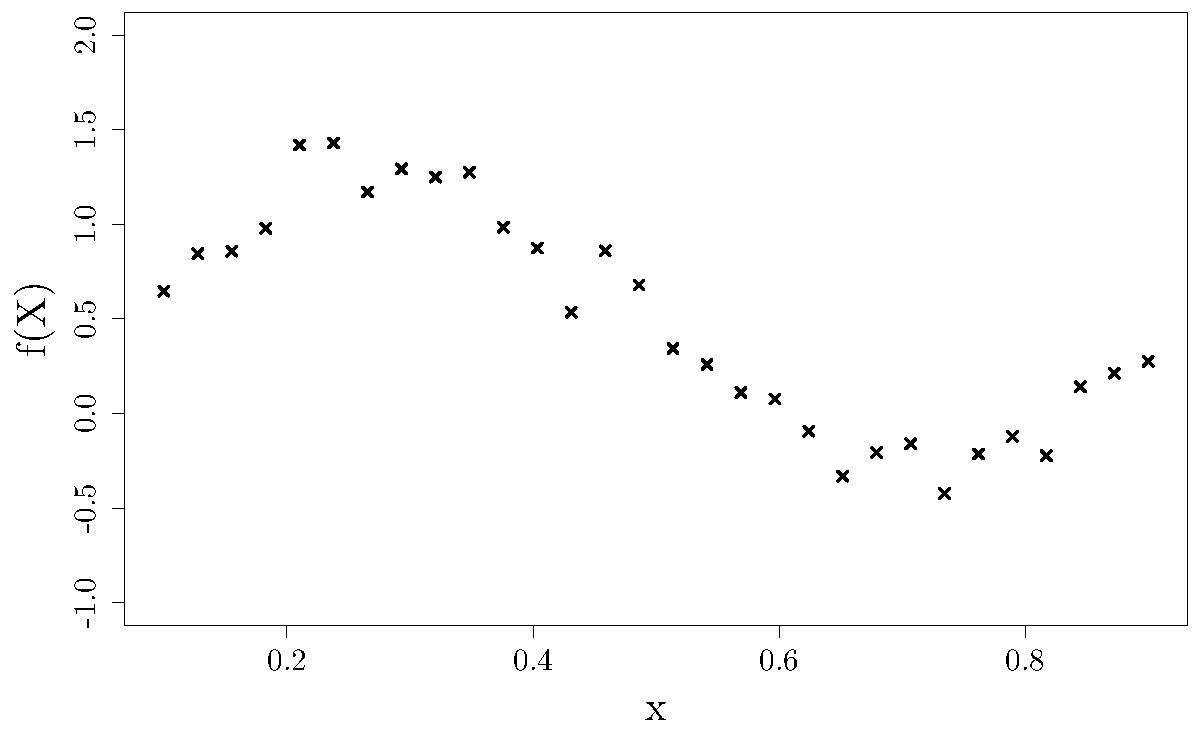
\includegraphics[height=6cm]{figures/R/noisyObs} 
\end{center}
\end{frame}

%%%%%%%%%%%%%%%%%%%%%%%%%%%%%%%%%%%%%%%%%%%%%%%%%%%%%%
\begin{frame}{}
\begin{exampleblock}{Exercise:}
	Let $f$ be a function of interest and let $F$ be a vector of ``noisy'' observations of $f$ at some input locations $X$:
	$$ F = f(X) + \varepsilon \text{\qquad with } \varepsilon \sim \mathcal{N}(0, \tau^2 Id). $$
	Let $Z$ be a Gaussian Process corresponding that can be used as prior distribution for $f$.
\begin{enumerate}
	\item Compute the conditional mean of $Z(x) | Z(X)+\varepsilon = F$
	\item Compute the conditional covariance function
\end{enumerate}
\end{exampleblock}
\end{frame}

%%%%%%%%%%%%%%%%%%%%%%%%%%%%%%%%%%%%%%%%%%%%%%%%%%%%%%
\begin{frame}{}
\begin{exampleblock}{Solution:}
\begin{enumerate}
	\item The conditional mean is
		\begin{equation*}
			\begin{split}
				m(x) &= \E[Z(x)|Z(X) + \varepsilon \shorteq F] \\
				&= k(x,X) (k(X,X)+ \tau^2 Id)^{-1} F \\ 
			\end{split}
		\end{equation*}
	\item The conditional variance is
		\begin{equation*}
			\begin{split}
				c(x,y) &= \Cov[Z(x),Z(y)|Z(X)+ \varepsilon \shorteq F] \\
				&= k(x,y) - k(x,X) (k(X,X)+\tau^2 Id)^{-1} k(X,y)
			\end{split}
		\end{equation*}
\end{enumerate}
\end{exampleblock}
Note that is si straightforward to generalize for a noise that is not i.i.d (as long as the noise is Gaussian distributed).
\end{frame}

%%%%%%%%%%%%%%%%%%%%%%%%%%%%%%%%%%%%%%%%%%%%%%%%%%%%%%
\begin{frame}{}
We obtain the following model
\begin{center}
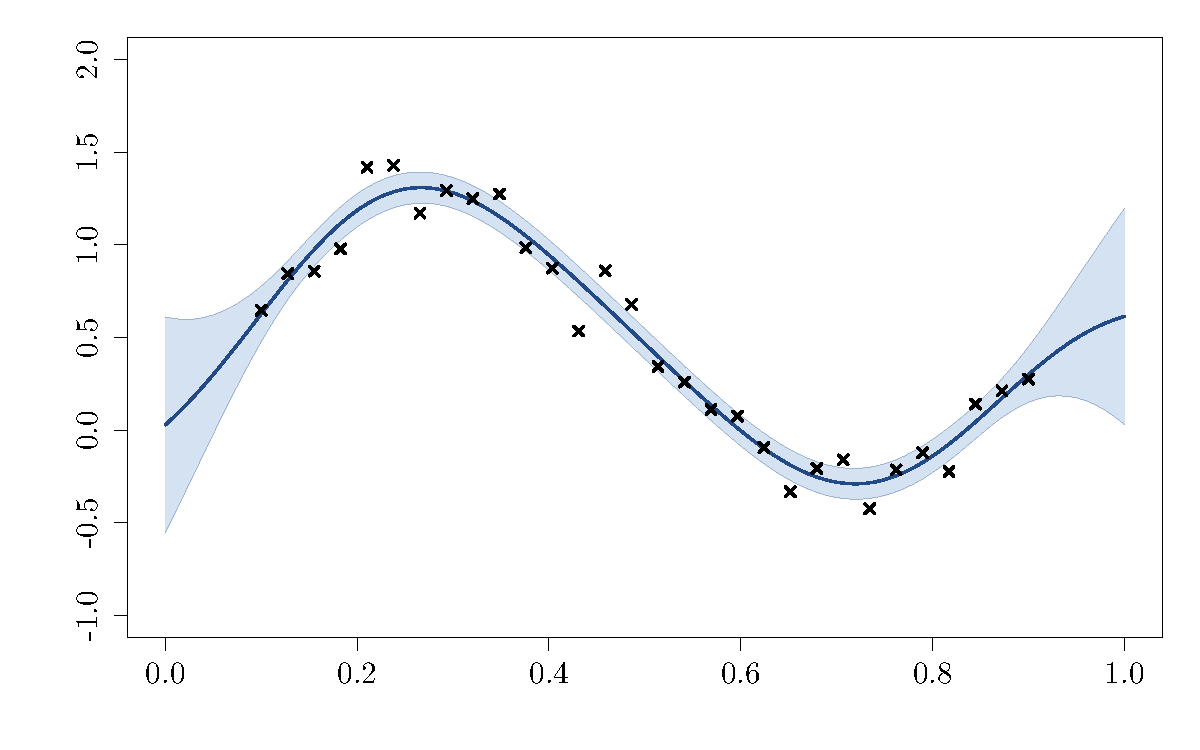
\includegraphics[height=6cm]{figures/R/noisyGPR} 
\end{center}
\end{frame}

%%%%%%%%%%%%%%%%%%%%%%%%%%%%%%%%%%%%%%%%%%%%%%%%%%%%%%
\begin{frame}{}
Influence of observation noise $\tau^2$:
\begin{center}
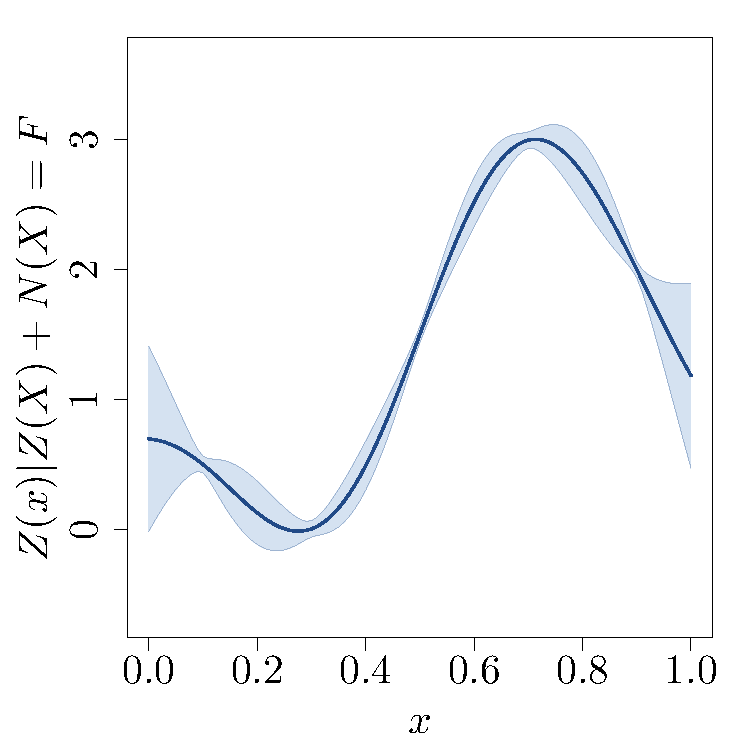
\includegraphics[height=3.5cm]{figures/R/ch34_GPRnoise0001} 
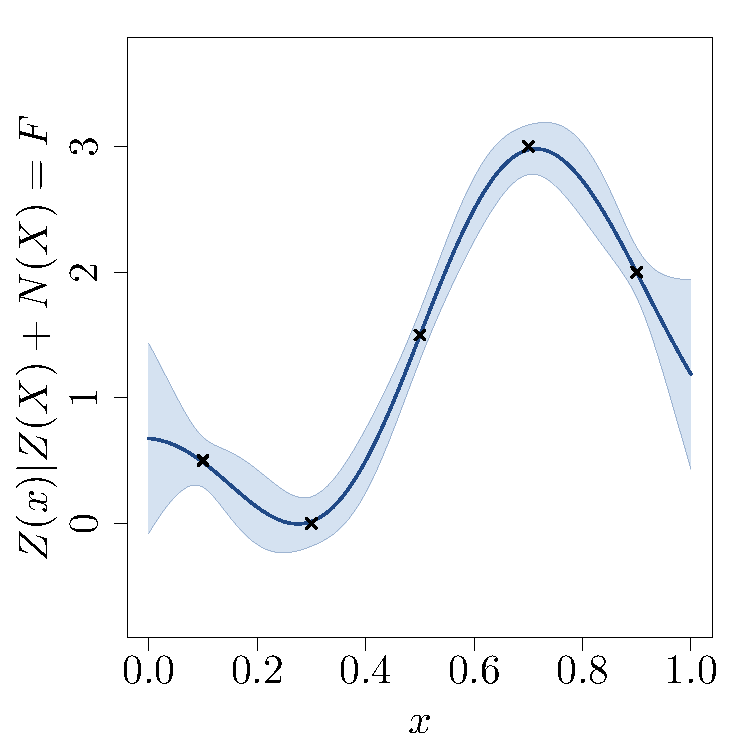
\includegraphics[height=3.5cm]{figures/R/ch34_GPRnoise001} 
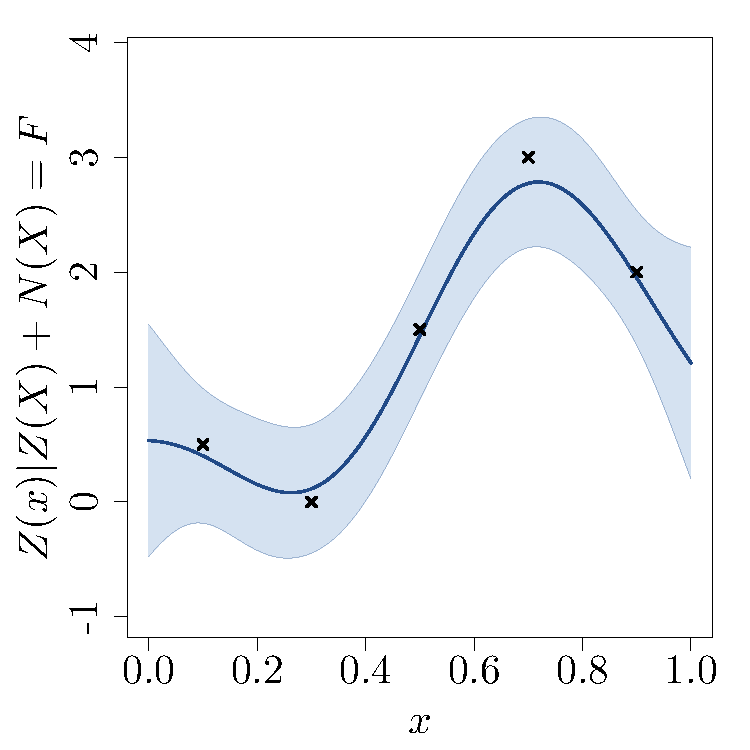
\includegraphics[height=3.5cm]{figures/R/ch34_GPRnoise01}\\
The values of $\tau^2$ are respectively 0.001, 0.01 and 0.1.
\end{center}
In practice, $\tau^2$ can be estimated with Maximum Likelihood. 
\end{frame}

%%%%%%%%%%%%%%%%%%%%%%%%%%%%%%%%%%%%%%%%%%%%%%%%%%%%%%%%%%%%%%%%%%%%%%%%
%%%%%%%%%%%%%%%%%%%%%%%%%%%%%%%%%%%%%%%%%%%%%%%%%%%%%%%%%%%%%%%%%%%%%%%%
\section{GPR in practice}
\subsection{}

%%%%%%%%%%%%%%%%%%%%%%%%%%%%%%%%%%%%%%%%%%%%%%%%%%%%%%
\begin{frame}{}
The various steps for building a GPR model are:\\ 
\vspace{3mm}
\begin{enumerate}
	\item Create a DoE
		\begin{itemize}
			\item What is the overall evaluation budget?
			\item What is my model for?
		\end{itemize} \vspace{2mm}
	\item Choose a kernel \vspace{3mm}
	\item Estimate the parameters
		\begin{itemize}
			\item Maximum likelihood
			\item Cross-validation
			\item Multi-start
		\end{itemize} \vspace{2mm}
	\item Validate the model 
		\begin{itemize}
			\item Test set 
			\item Leave-one-out to check mean and confidence intervals
			\item Leave-$k$-out to check predicted covariances
		\end{itemize}
\end{enumerate}
\begin{exampleblock}{Remarks}
	\begin{itemize}
		\item It is common to iterate over steps 2, 3 and 4.
	\end{itemize}
\end{exampleblock}
\end{frame}


%%%%%%%%%%%%%%%%%%%%%%%%%%%%%%%%%%%%%%%%%%%%%%%%%%%%%%
\begin{frame}{}
In practice, the following errors may appear:\\
\begin{itemize}
	\item[\alert{$\bullet$}] \alert{Error: the matrix is not invertible}
	\item[\alert{$\bullet$}] \alert{Error: the matrix is not positive definite}
\end{itemize}
Covariance matrices are positive semi-definite. Null eigenvalues arise if one information is repeated.
\begin{example}
 For $X=(0.1,0.1,0.4,0.6,0.8)$, the covariance of a squared exponential kernel with parameters $\sigma^2=1$, $\theta = 0.2$ is: 
 \begin{equation*}
 k(X,X) = 
 \begin{pmatrix}
	1.00 & 1.00 & 0.32 & 0.04 & 0.00 \\
	1.00 & 1.00 & 0.32 & 0.04 & 0.00 \\
	0.32 & 0.32 & 1.00 & 0.61 & 0.14 \\
	0.04 & 0.04 & 0.61 & 1.00 & 0.61 \\
	0.00 & 0.00 & 0.14 & 0.61 & 1.00 \\
 \end{pmatrix}
 \end{equation*}
 The first two columns are the same, so the matrix is not invertible.
\end{example}
\end{frame}

%%%%%%%%%%%%%%%%%%%%%%%%%%%%%%%%%%%%%%%%%%%%%%%%%%%%%%
\begin{frame}{}
It is particularly interesting to look at the eigenvectors associated with null eigenvalues. On the previous example, this eigenvector is 
\begin{equation*}
P_0 = \left( \frac{1}{\sqrt{2}},-\frac{1}{\sqrt{2}},0,0,0 \right)^t
\end{equation*}
Now, 2 situations can be distinguished\\ \vspace{2mm}
\begin{itemize}
	\item[(A)] The observations are compatible with the model: $P_0^t F = 0$.
	\begin{itemize}
		\item the model is appropriate and one observation can be removed without any loss of information.
	\end{itemize}
	\item[(B)] The obs. \textbf{are not} compatible with the model: $P_0^t F \neq 0$.
		\begin{itemize}
			\item the model is not appropriate and it should be modified. For example, observation noise can be added.
		\end{itemize}
\end{itemize}
In both cases, the covariance matrix will become invertible.
\end{frame}

%%%%%%%%%%%%%%%%%%%%%%%%%%%%%%%%%%%%%%%%%%%%%%%%%%%%%%
\begin{frame}{}
In practice, invertibility issues may arise if observations points are close-by. \\
\vspace{3mm}
This is specially true if
\begin{itemize}
	\item the kernel corresponds to very regular sample paths (squared-exponential for example)
	\item the range (or length-scale) parameters are large
\end{itemize}
\vspace{3mm}
In order to avoid numerical problems during optimization, one can:
\begin{itemize}
	\item add a (very) small observation noise\\
	\item impose a maximum bound to length-scales
	\item impose a minimal bound for noise variance 
	\item choose a Mat\'ern kernel
\end{itemize}
\end{frame}

%%%%%%%%%%%%%%%%%%%%%%%%%%%%%%%%%%%%%%%%%%%%%%%%%%%%%%
\begin{frame}{}
A few words on GPR \textbf{Complexity}\\ \vspace{2mm}
	\begin{itemize}
  		\item \structure{Storage footprint:} We have to store the covariance matrix which is $n \times n$.
  		\item \structure{Complexity:} We have to invert the covariance matrix, which requires is $\mathcal{O}(n^3)$.\\
	\end{itemize}
Storage footprint is often the first limit to be reached.\\
\vspace{5mm}
The maximal number of observation points is between $1000$ and $10\,000$.\\
\vspace{2mm}
Note that the complexity do not depend on the dimension of the input space!
\end{frame}

%%%%%%%%%%%%%%%%%%%%%%%%%%%%%%%%%%%%%%%%%%%%%%%%%%%%%%
%%%%%%%%%%%%%%%%%%%%%%%%%%%%%%%%%%%%%%%%%%%%%%%%%%%%%%
\section{GPR with trend}
\subsection{}

%%%%%%%%%%%%%%%%%%%%%%%%%%%%%%%%%%%%%%%%%%%%%%%%%%%%%%
\begin{frame}{}
We have seen that GPR models go back to zero if we consider a centred prior. \\ \vspace{5mm} This behaviour is not always wanted
\begin{center}
	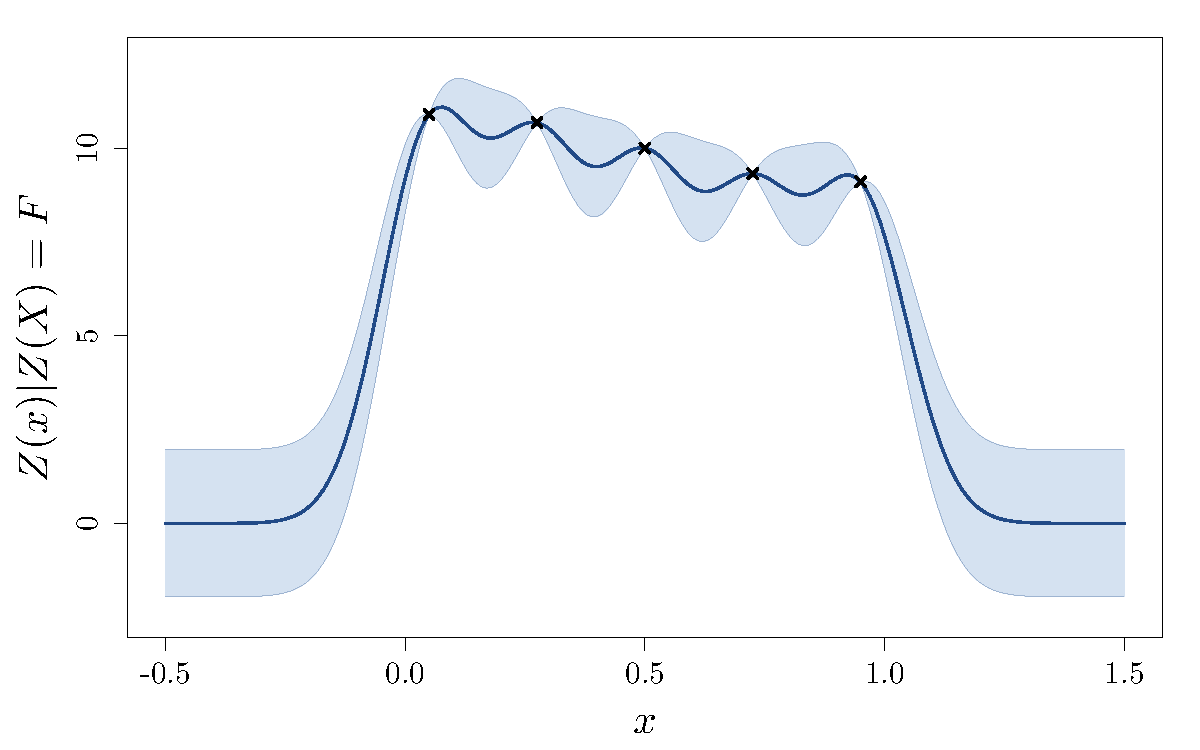
\includegraphics[height=5cm]{figures/R/trend_pb}
\end{center}
\end{frame}

%%%%%%%%%%%%%%%%%%%%%%%%%%%%%%%%%%%%%%%%%%%%%%%%%%%%%%
\begin{frame}{}
If the trend $t(.)$ is known, the usual formulas for multivariate normal conditional distribution apply:
\begin{equation*}
	\begin{split}
		m(x) &= \E[Z(x)|Z(X) \shorteq F] \\
		&= t(x) + k(x,X) k(X,X)^{-1} (F-t(X)) \\ \vspace{3mm}
		c(x,y) &= \Cov[Z(x),Z(y)|Z(X) \shorteq F] \\
		&= k(x,y) - k(x,X) k(X,X)^{-1} k(X,y)
	\end{split}
\end{equation*}
We can see that the trend is subtracted first and then added in the end.
\end{frame}

%%%%%%%%%%%%%%%%%%%%%%%%%%%%%%%%%%%%%%%%%%%%%%%%%%%%%%
\begin{frame}{}
In the previous example, we can consider that trend is constant $t(x)=10$:
\begin{center}
	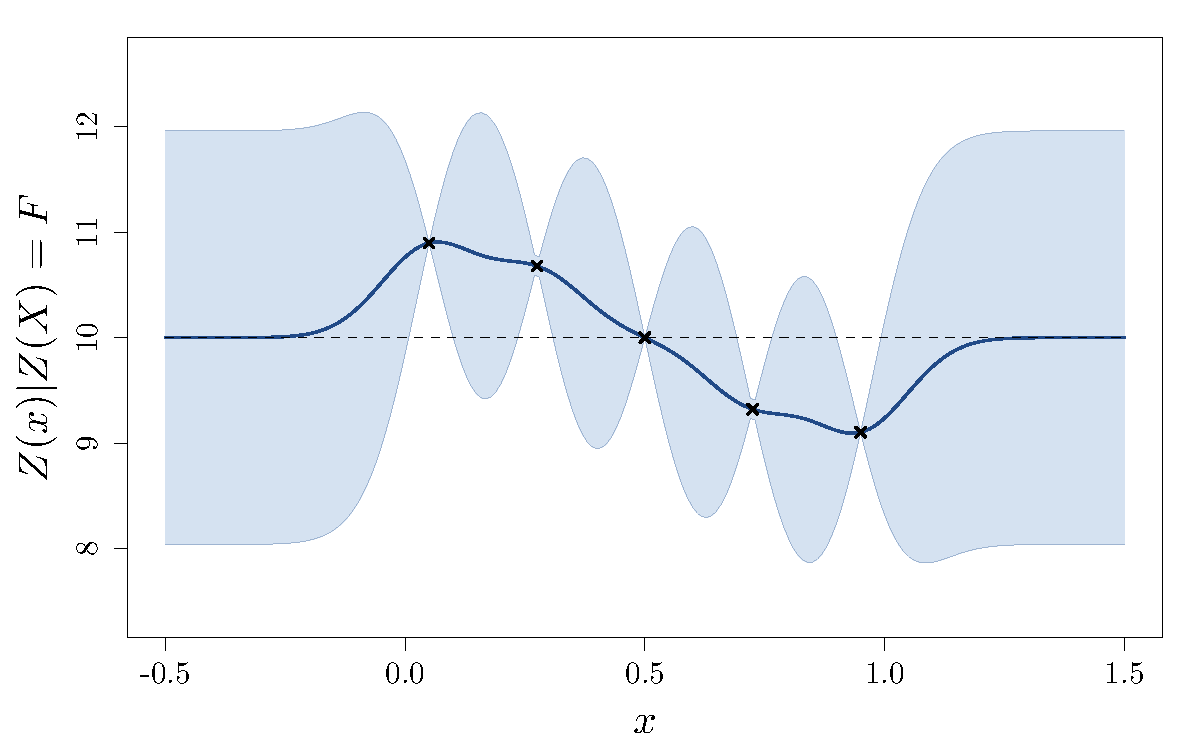
\includegraphics[height=6cm]{figures/R/trend_knowncst}
\end{center}
\end{frame}

%%%%%%%%%%%%%%%%%%%%%%%%%%%%%%%%%%%%%%%%%%%%%%%%%%%%%%
\begin{frame}{}
We can also try a linear trend $t(x)=11-2x$:
\begin{center}
	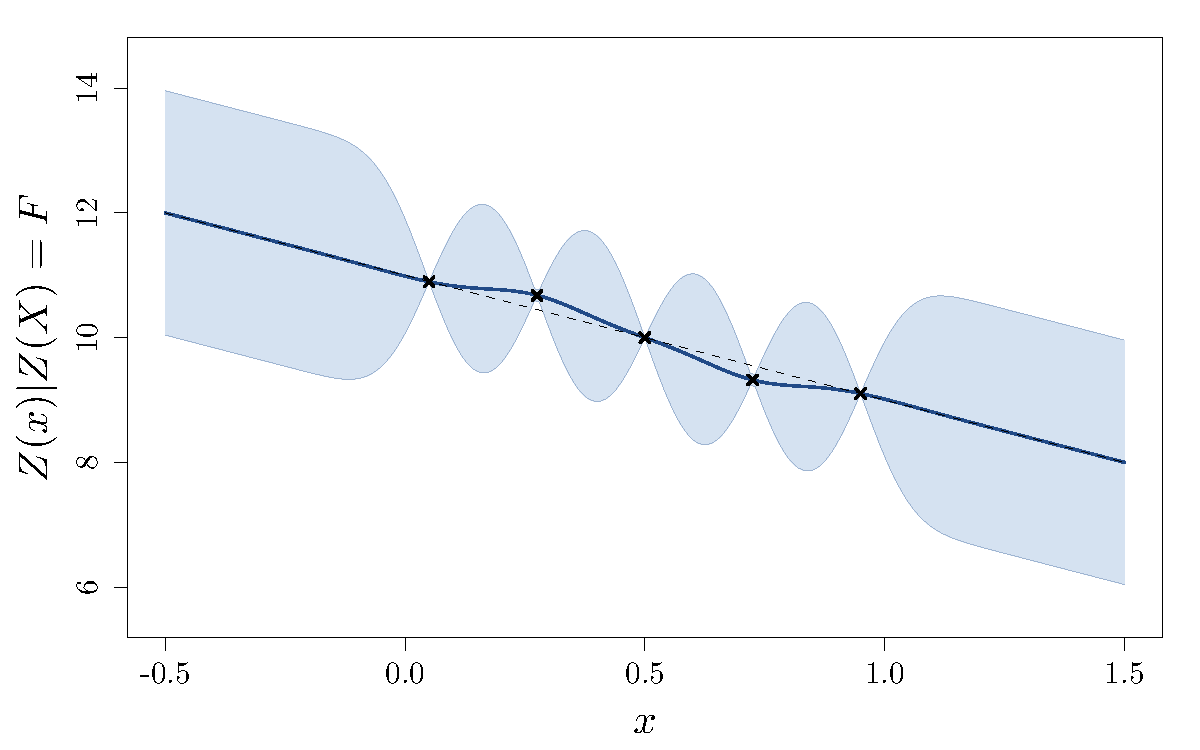
\includegraphics[height=6cm]{figures/R/trend_knownlin}
\end{center}
\end{frame}

%%%%%%%%%%%%%%%%%%%%%%%%%%%%%%%%%%%%%%%%%%%%%%%%%%%%%%
\begin{frame}{}
In practice, the trend is often unknown... The question is then how to estimate it.\\ \vspace{5mm} 
We will distinguish:
\begin{itemize}
	\item \textbf{simple kriging}: there is no trend or it is known
	\item \textbf{ordinary kriging}: the trend is a constant
	\item \textbf{universal kriging}: the trend is given by basis functions
\end{itemize}
\end{frame}

%%%%%%%%%%%%%%%%%%%%%%%%%%%%%%%%%%%%%%%%%%%%%%%%%%%%%%
\begin{frame}{}
We will first focus on \textbf{ordinary kriging}. We thus need to estimate a constant:\\ \vspace{5mm} 
\begin{center}
	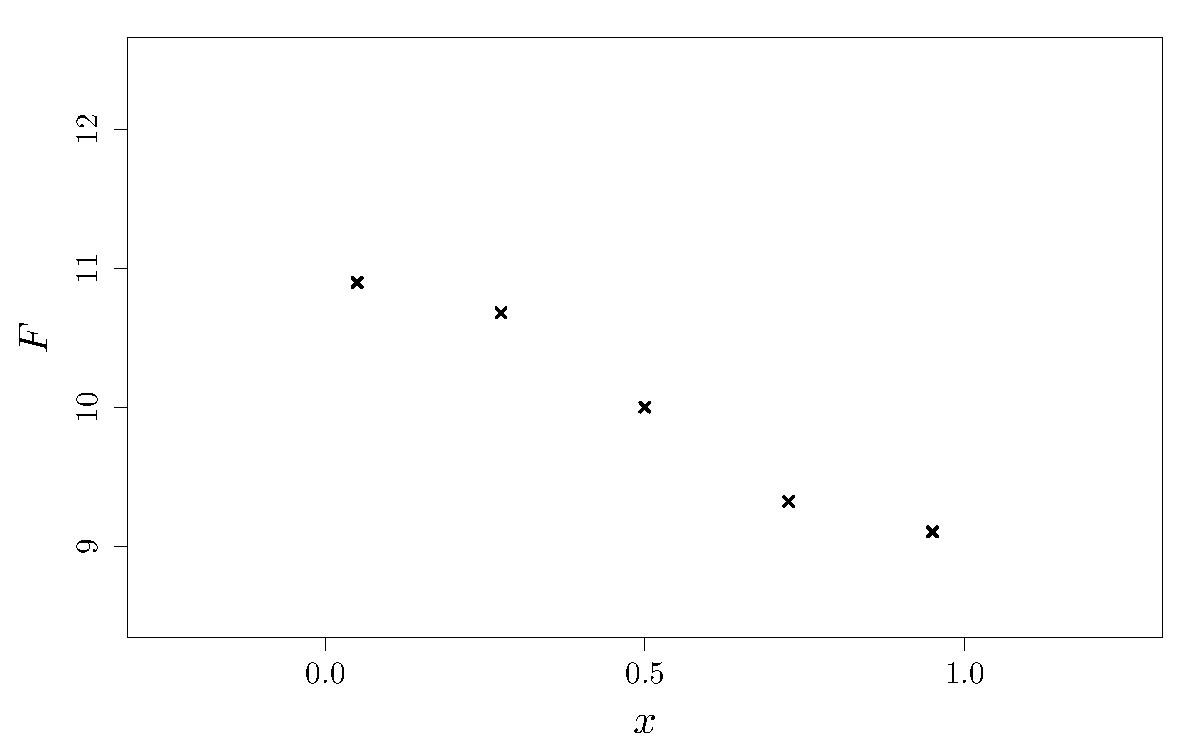
\includegraphics[height=6cm]{figures/R/trend_dataordinary}
\end{center}
\end{frame}

%%%%%%%%%%%%%%%%%%%%%%%%%%%%%%%%%%%%%%%%%%%%%%%%%%%%%%
\begin{frame}{}
The idea of considering $t(x)=\text{mean}(F)$ looks all right on this example...
\begin{center}
	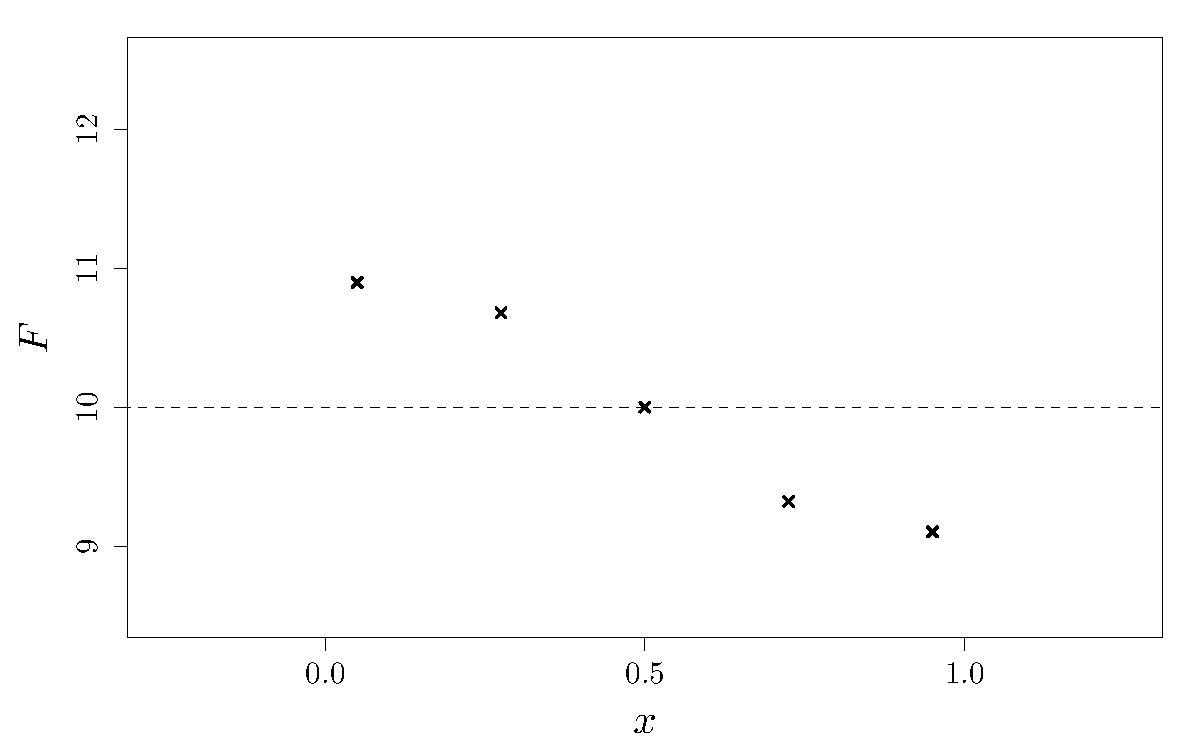
\includegraphics[height=6cm]{figures/R/trend_basicordinary}
\end{center}
\end{frame}

%%%%%%%%%%%%%%%%%%%%%%%%%%%%%%%%%%%%%%%%%%%%%%%%%%%%%%
\begin{frame}{}
but not on this one.
\begin{center}
	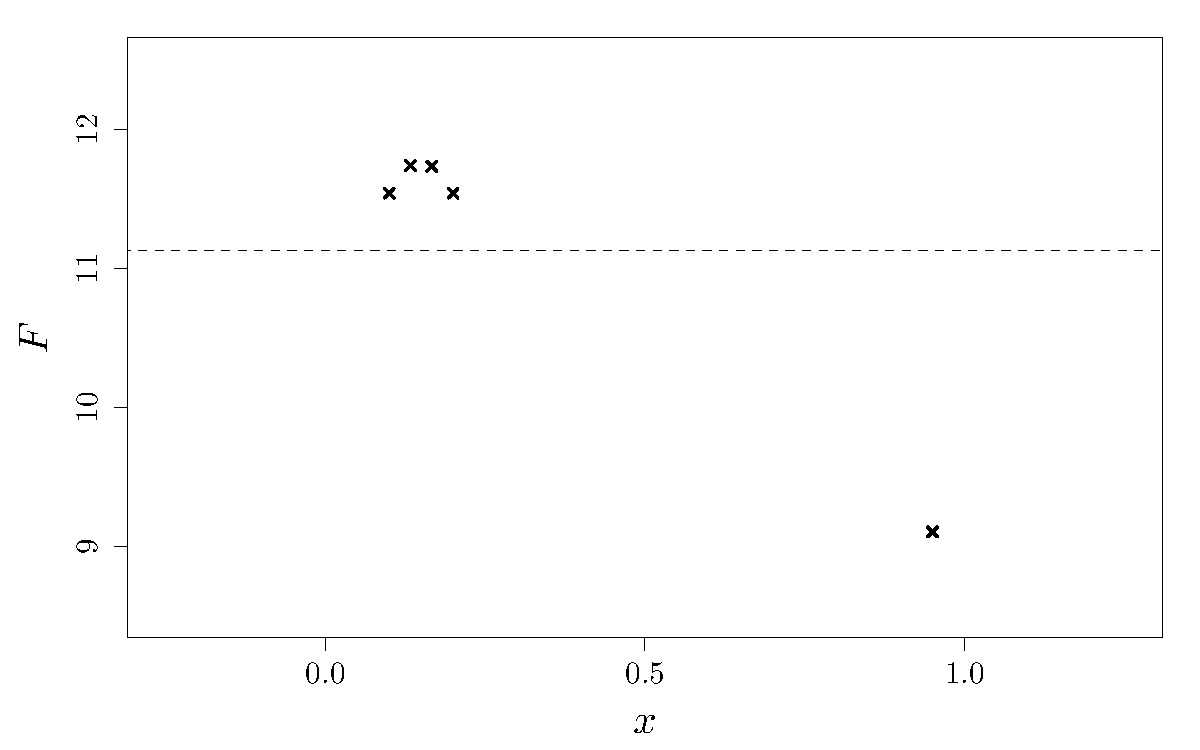
\includegraphics[height=6cm]{figures/R/trend_pbbasicordinary}
\end{center}
Any other idea?
\end{frame}

%%%%%%%%%%%%%%%%%%%%%%%%%%%%%%%%%%%%%%%%%%%%%%%%%%%%%%
\begin{frame}{}
We have considered maximum likelihood estimation for the kernel's parameter... why not doing the same thing here ?
\begin{exampleblock}{Exercise}
\begin{enumerate}
	\item Compute the maximum likelihood estimation $\hat{t}$ of $t$. A few hints
	\begin{itemize}
		\item consider the log-likelihood
		\item take the derivative
		\item find where it is null
	\end{itemize}
	\item What can we recognize in this expression ?
\end{enumerate}
We recall that the likelihood is
\begin{equation*}
L(t) = \frac{1}{\displaystyle (2 \pi)^{n/2} |k(X,X)|^{1/2}} \exp \left(-\frac12 (F-t \mathbf{1})^t k(X,X)^{-1} (F-t \mathbf{1})  \right)
\end{equation*}
\end{exampleblock}
\end{frame}

%%%%%%%%%%%%%%%%%%%%%%%%%%%%%%%%%%%%%%%%%%%%%%%%%%%%%%
\begin{frame}{}
\begin{exampleblock}{Solution}
\begin{enumerate}
	\item We obtain $ \displaystyle \hat{t} = \frac{\mathbf{1}^t k(X,X)^{-1} F}{\mathbf{1}^t k(X,X)^{-1} \mathbf{1}}$ 
	\item It can be seen as an orthogonal projection $ \displaystyle t = \frac{\PSi{\mathbf{1}, F}{}}{\PSi{\mathbf{1},\mathbf{1}}{}}$ for a inner product given by 
	$k(X,X)^{-1}$. 
\end{enumerate}
\end{exampleblock}
\begin{columns}[c]
\begin{column}{4cm}
On the previous example we obtain $t=10.3$:
\end{column}
\begin{column}{6cm}
\hspace{-8mm} 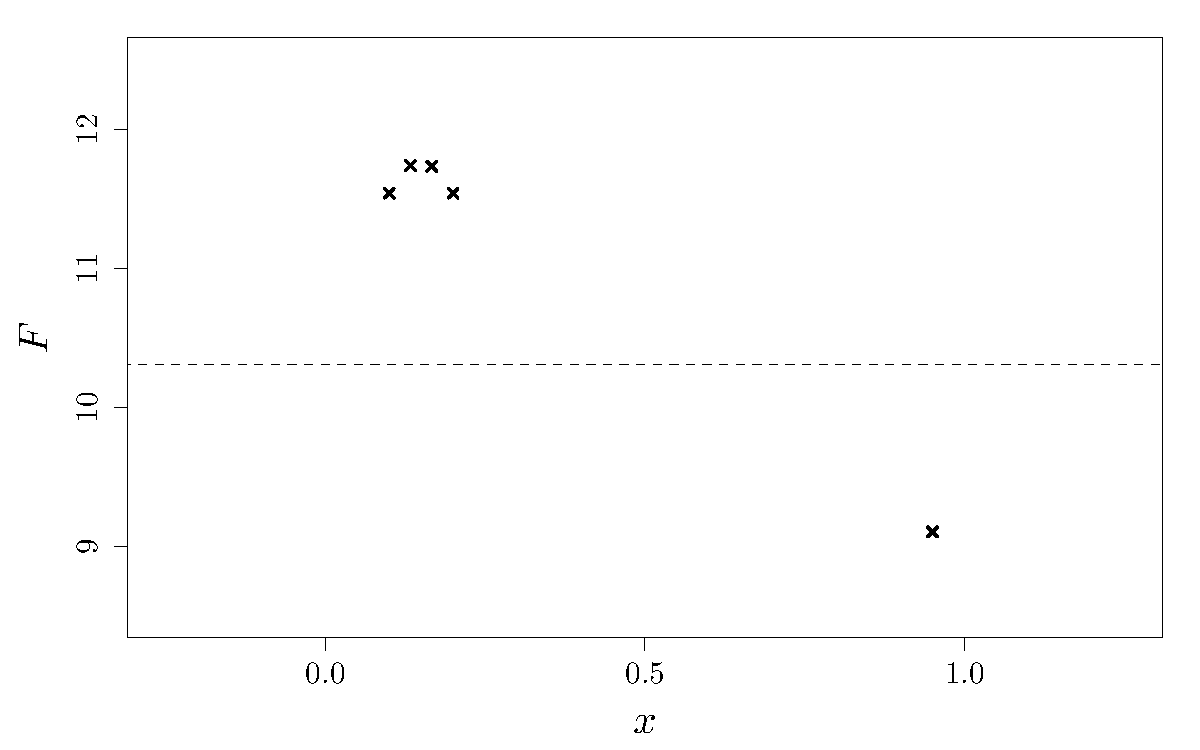
\includegraphics[height=4.2cm]{figures/R/trend_estimordinary}
\end{column}
\end{columns}
\end{frame}

%%%%%%%%%%%%%%%%%%%%%%%%%%%%%%%%%%%%%%%%%%%%%%%%%%%%%%
\begin{frame}{}
Under the hypothesis $F=Z(X)$, the estimation $ \displaystyle \hat{t} = \frac{\mathbf{1}^t k(X,X)^{-1} F}{\mathbf{1}^t k(X,X)^{-1} \mathbf{1}}$ is a sample from $ \displaystyle T = \frac{\mathbf{1}^t k(X,X)^{-1} Z(X)}{\mathbf{1}^t k(X,X)^{-1} \mathbf{1}}$. \\ \vspace{5mm}
The distribution of $T$ is Gaussian with moments:
\begin{equation*}
\begin{split}
	\E[T] & = \frac{\mathbf{1}^t k(X,X)^{-1} \E[Z(X)]}{\mathbf{1}^t k(X,X)^{-1} \mathbf{1}} = t\\
	\Var[T] & = \frac{\mathbf{1}^t k(X,X)^{-1} \Var[Z(X)] k(X,X)^{-1} \mathbf{1}}{(\mathbf{1}^t k(X,X)^{-1} \mathbf{1})^2} = \frac{1}{\mathbf{1}^t k(X,X)^{-1} \mathbf{1}}\\
\end{split}
\end{equation*}
\end{frame}

%%%%%%%%%%%%%%%%%%%%%%%%%%%%%%%%%%%%%%%%%%%%%%%%%%%%%%
\begin{frame}{}
The expression of the \textbf{best predictor} is given by the usual conditioning of a GP:
\begin{equation*}
m(x) = \E[Z(x)|Z(X)=F] = \hat{t} - k(x,X) k(X,X)^{-1} (F - \hat{t}) \vspace{5mm}
\end{equation*} 

Regarding the \textbf{model variance}, it must account for the estimator's variance. We will use the law of total Variance :
\begin{equation*}
\Var[X] = \E[\Var(X|Y)] + \Var[\E(X|Y)]
\end{equation*} 
If we apply this to the GPR variance prediction we get:
\small
\begin{equation*}
\begin{split}
\Var[Z(x)|Z(X)] &=  k(x,x) - k(x,X) k(X,X)^{-1} k(X,x)   \\
& \qquad + \frac{(\mathbf{1} + k(x,X)k(X,X)^{-1}\mathbf{1})^t(\mathbf{1} + k(x,X)k(X,X)^{-1}\mathbf{1})}{\mathbf{1}^t k(X,X)^{-1} \mathbf{1}} \\
\end{split}
\end{equation*} 
\normalsize
\end{frame}

%%%%%%%%%%%%%%%%%%%%%%%%%%%%%%%%%%%%%%%%%%%%%%%%%%%%%%
\begin{frame}{}
On the previous example we obtain:
\begin{center}
	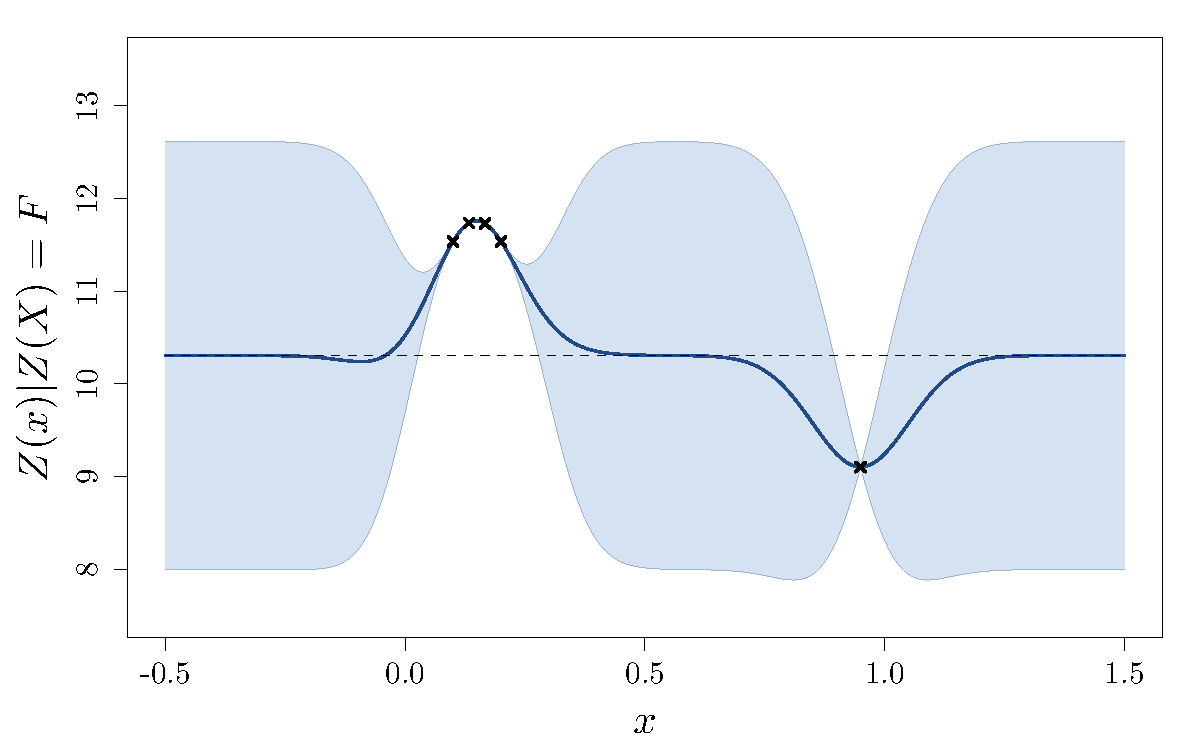
\includegraphics[height=6cm]{figures/R/trend_ko}
\end{center}
\end{frame}

%%%%%%%%%%%%%%%%%%%%%%%%%%%%%%%%%%%%%%%%%%%%%%%%%%%%%%
\begin{frame}{}
We would have obtain this the mean were considered known.
\begin{center}
	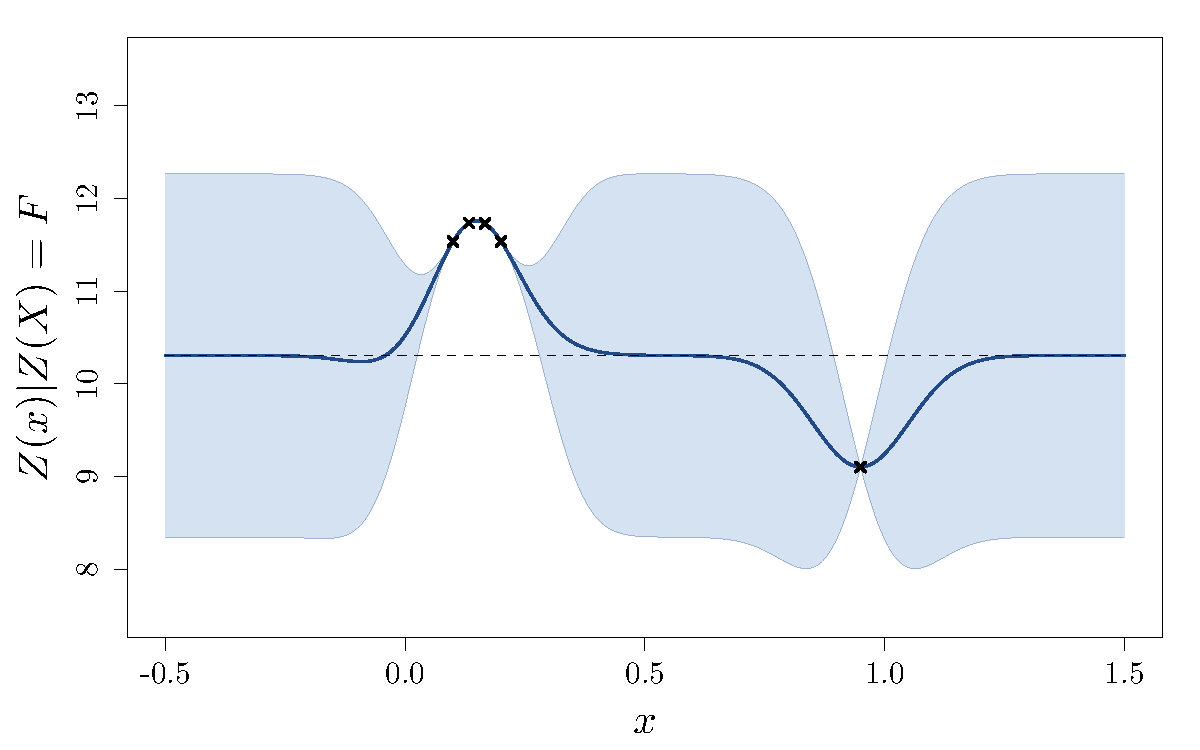
\includegraphics[height=6cm]{figures/R/trend_badko}
\end{center}
\end{frame}

%%%%%%%%%%%%%%%%%%%%%%%%%%%%%%%%%%%%%%%%%%%%%%%%%%%%%%
\begin{frame}{}
it can be compared with simple kriging
\begin{center}
	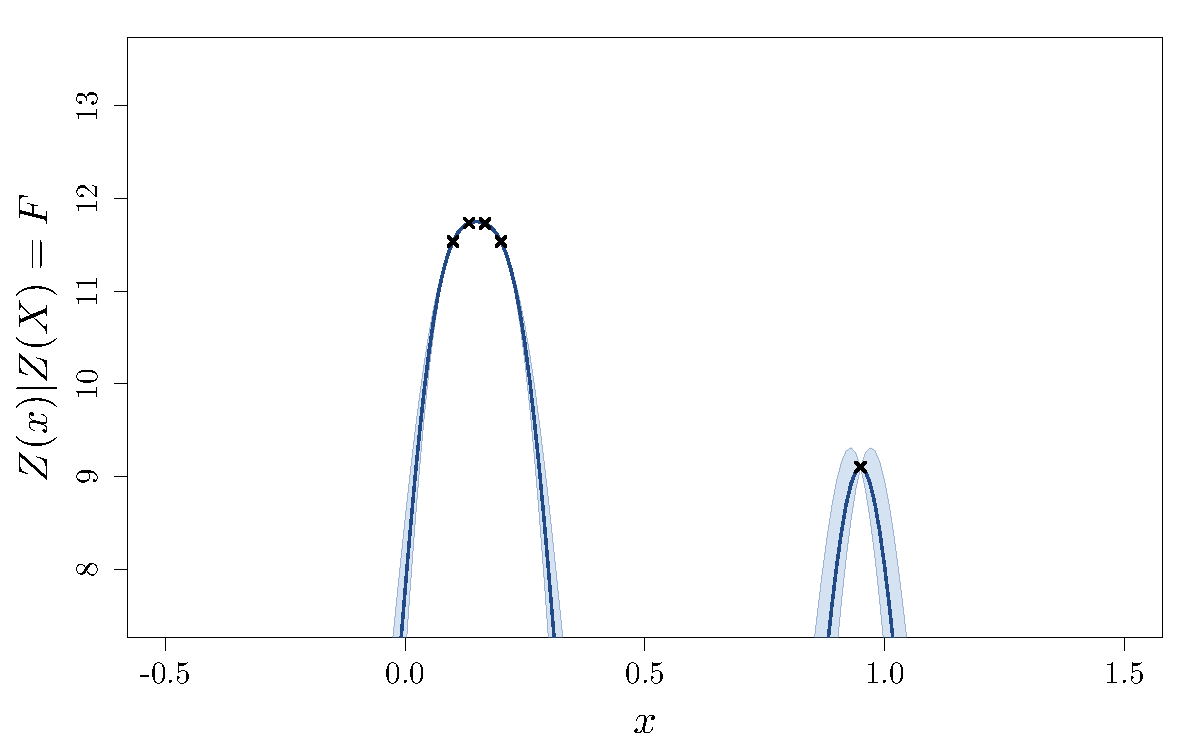
\includegraphics[height=6cm]{figures/R/trend_badks}
\end{center}
\end{frame}

%%%%%%%%%%%%%%%%%%%%%%%%%%%%%%%%%%%%%%%%%%%%%%%%%%%%%%
\begin{frame}{}
If the trend is not constant but linear, quadratic, etc. it is interesting to consider the following probabilistic model for the prior:
\begin{equation*}
	Z(x) = Y(x) + \sum_i \beta_i h_i(x)
\end{equation*}
where the $h_i(x)$ are basis functions and the $\beta_i$ are unknown scalars.\\ \vspace{5mm}
As previously, we can consider the maximum likelihood estimator 
\begin{equation*}
 \hat{\beta} = (H^t k(X,X)^{-1} H)^{-1} H^t k(X,X)^{-1} F 
\end{equation*} 
where $H$ is the matrix of general term $H_{i,j}=h_j(X_i)$.
\end{frame}

%%%%%%%%%%%%%%%%%%%%%%%%%%%%%%%%%%%%%%%%%%%%%%%%%%%%%%
\begin{frame}{}
The final equations are very similar to ordinary kriging:
\begin{block}{Universal kriging}
\begin{equation*}
\begin{split}
m(x) &= h(x)^t\hat{\beta} - k_x K^{-1} (F - h(X)^t\hat{\beta}) \\
c(x,y) &=  k(x,y) - k_x K^{-1} k_y^t \\
& \qquad +(h(x)^t + k_xK^{-1}H)^t(H^t K^{-1} H)^{-1}(h(y)^t + k_yK^{-1}H) \\
\end{split}
\end{equation*} 
\\ \vspace{3mm}
where $k_x = k(x,X)$ and $K = k(X,X)$.
\end{block}
\end{frame}

%%%%%%%%%%%%%%%%%%%%%%%%%%%%%%%%%%%%%%%%%%%%%%%%%%%%%%
\begin{frame}{}
\structure{Remarks}
\begin{itemize}
	\item Ordinary kriging is a special case of universal kriging with only one constant basis function.
	\item The model always interpolates whatever $\hat{\beta}$ is.
	\item the trend part can be seen as generalised least square (regression with correlated residuals)
\end{itemize}
\end{frame}

%%%%%%%%%%%%%%%%%%%%%%%%%%%%%%%%%%%%%%%%%%%%%%%%%%%%%%
\begin{frame}{}
We consider the following example
\begin{center}
	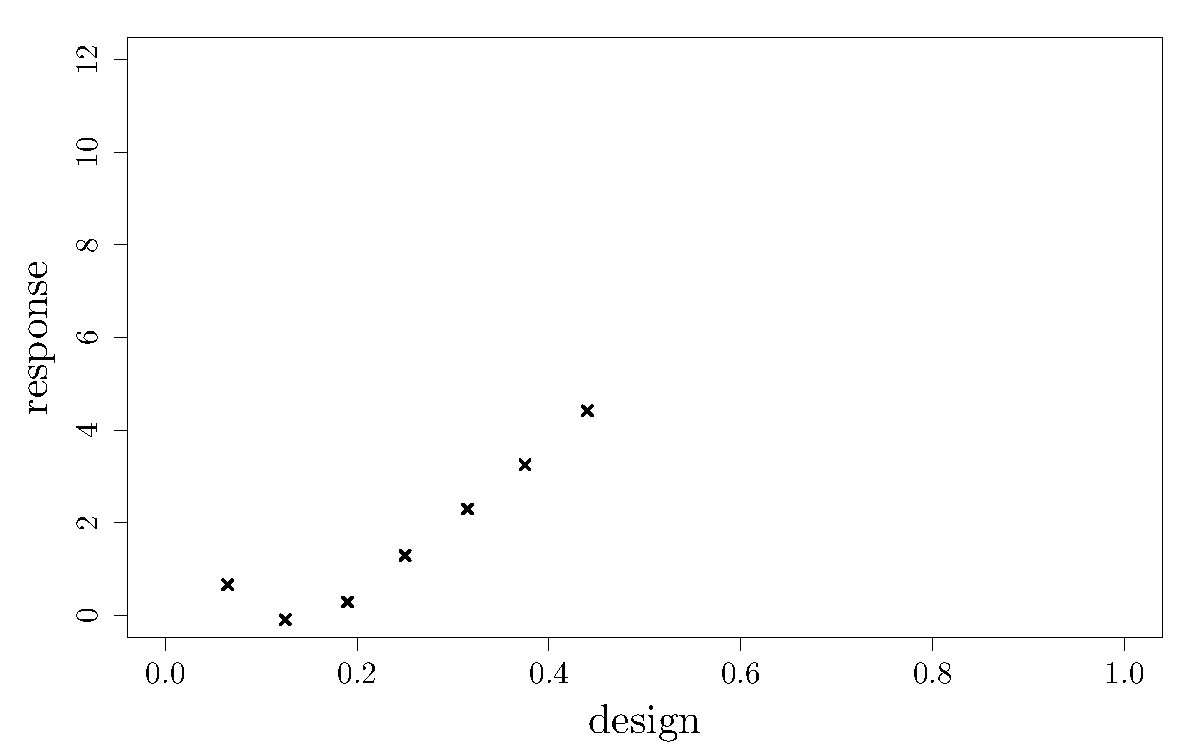
\includegraphics[height=6cm]{figures/R/trend_data}
\end{center}
\end{frame}

%%%%%%%%%%%%%%%%%%%%%%%%%%%%%%%%%%%%%%%%%%%%%%%%%%%%%%
\begin{frame}{}
Universal kriging model with linear trend: $h_1(x) = 1$, $h_2(x) = x$.
\begin{center}
	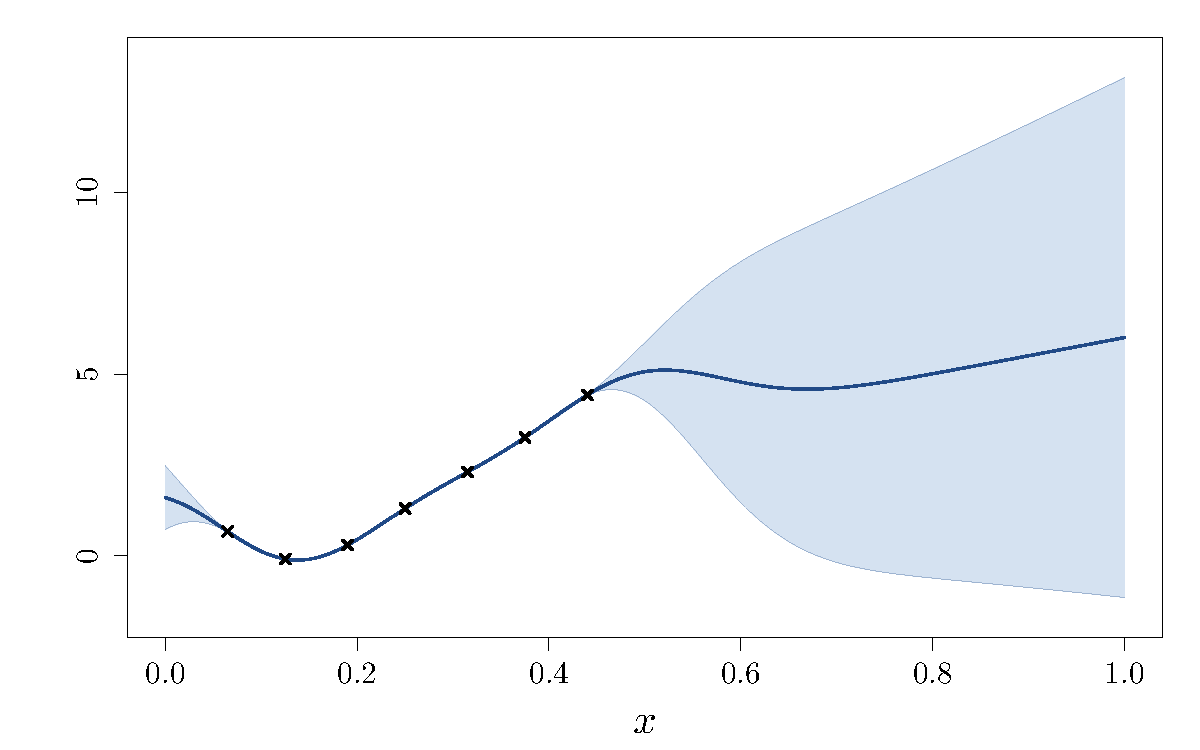
\includegraphics[height=6cm]{figures/R/trend_ku}
\end{center}
\end{frame}

%%%%%%%%%%%%%%%%%%%%%%%%%%%%%%%%%%%%%%%%%%%%%%%%%%%%%%
\begin{frame}{}
It can be compared to simple kriging with known trend
\begin{center}
	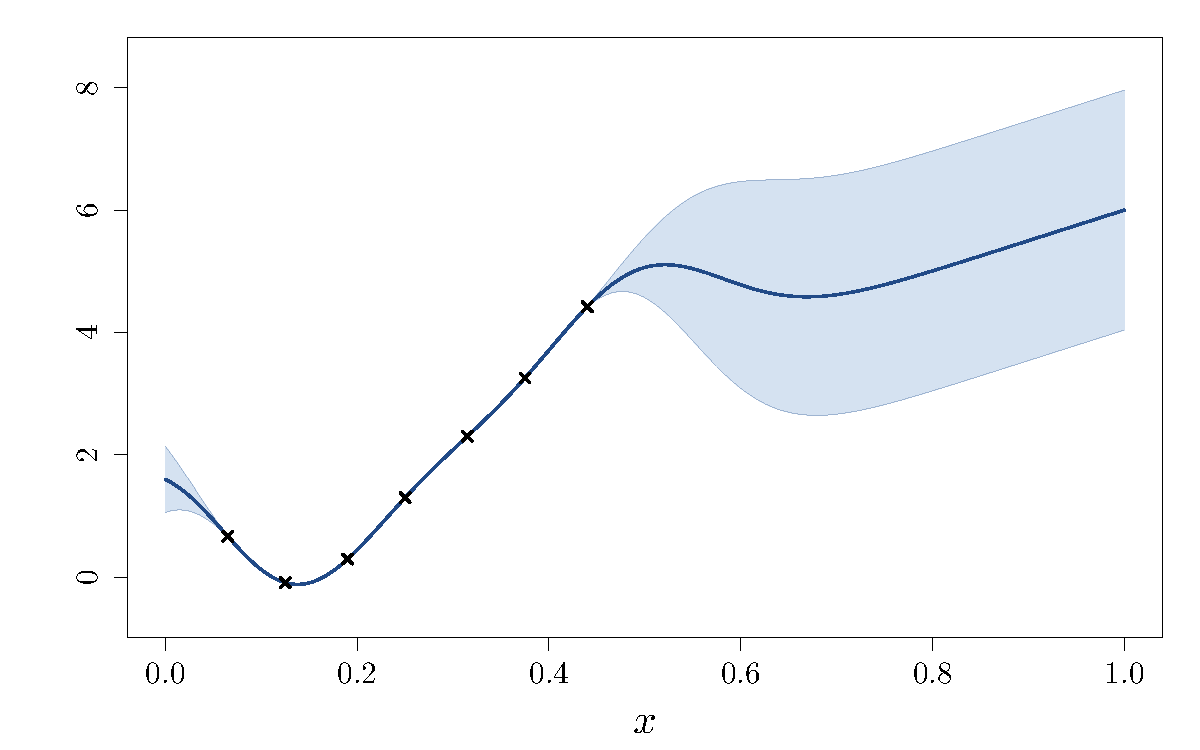
\includegraphics[height=6cm]{figures/R/trend_kstrend}
\end{center}
\end{frame}

%%%%%%%%%%%%%%%%%%%%%%%%%%%%%%%%%%%%%%%%%%%%%%%%%%%%%%%%%%%%%%%%%%%%%%%%%%%%%%%%%%%%
%%%%%%%%%%%%%%%%%%%%%%%%%%%%%%%%%%%%%%%%%%%%%%%%%%%%%%%%%%%%%%%%%%%%%%%%%%%%%%%%%%%%
\section{Making new from old}
\subsection{}


% %%%%%%%%%%%%%%%%%%%%%%%%%%%%%%%%%%%%%%%%%%%%%%%%%%%%%%
% \begin{frame}{}
% We have seen that it is difficult to prove directly the positive semi-definiteness of a function. \\
% \begin{block}{}
% \textbf{For all} $n \in \mathds{N}$,  \textbf{for all} $x_i \in D$,  \textbf{for all} $a_i \in \mathds{R}$ 
% \begin{equation*}
% \sum \sum a_i  a_j K(x_i,x_j) \geq 0
% \end{equation*}
% \end{block} \ \\ 
% However, many operations can be applied to a psd function while retaining this property. This is often called \structure{making new from old}.
% \end{frame}


%%%%%%%%%%%%%%%%%%%%%%%%%%%%%%%%%%%%%%%%%%%%%%%%%%%%%%
\begin{frame}{}
\structure{Making new from old:}
\begin{block}{}
Kernels can be:
\begin{itemize}
  \item Summed together
  \begin{itemize}
    \item On the same space $k(x,y) = k_1(x,y) + k_2(x,y)$
    \item On the tensor space $k(\mathbf{x},\mathbf{y}) = k_1(x_1,y_1) + k_2(x_2,y_2)$
  \end{itemize} 
  \item Multiplied together
  \begin{itemize}
    \item On the same space $k(x,y) = k_1(x,y) \times k_2(x,y)$
    \item On the tensor space $k(\mathbf{x},\mathbf{y}) = k_1(x_1,y_1) \times k_2(x_2,y_2)$
  \end{itemize} 
  \item Composed with a function
  \begin{itemize}
    \item $k(x,y) = k_1(f(x),f(y))$
  \end{itemize} 
\end{itemize} 
\end{block}
All these operations will preserve the positive definiteness.\\ 
\vspace{0.2cm}
\begin{center}
\alert{How can this be useful?}
\end{center}
\end{frame}

%%%%%%%%%%%%%%%%%%%%%%%%%%%%%%%%%%%%%%%%%%%%%%%%%%%%%%
%%%%%%%%%%%%%%%%%%%%%%%%%%%%%%%%%%%%%%%%%%%%%%%%%%%%%%
%\subsection{Sum of kernels}

%%%%%%%%%%%%%%%%%%%%%%%%%%%%%%%%%%%%%%%%%%%%%%%%%%%%%%
\begin{frame}{Sum of kernels over the same space }
\begin{example}[The Mauna Loa observatory dataset]
This famous dataset compiles the monthly $CO_2$ concentration in Hawaii since 1958.
\begin{center}
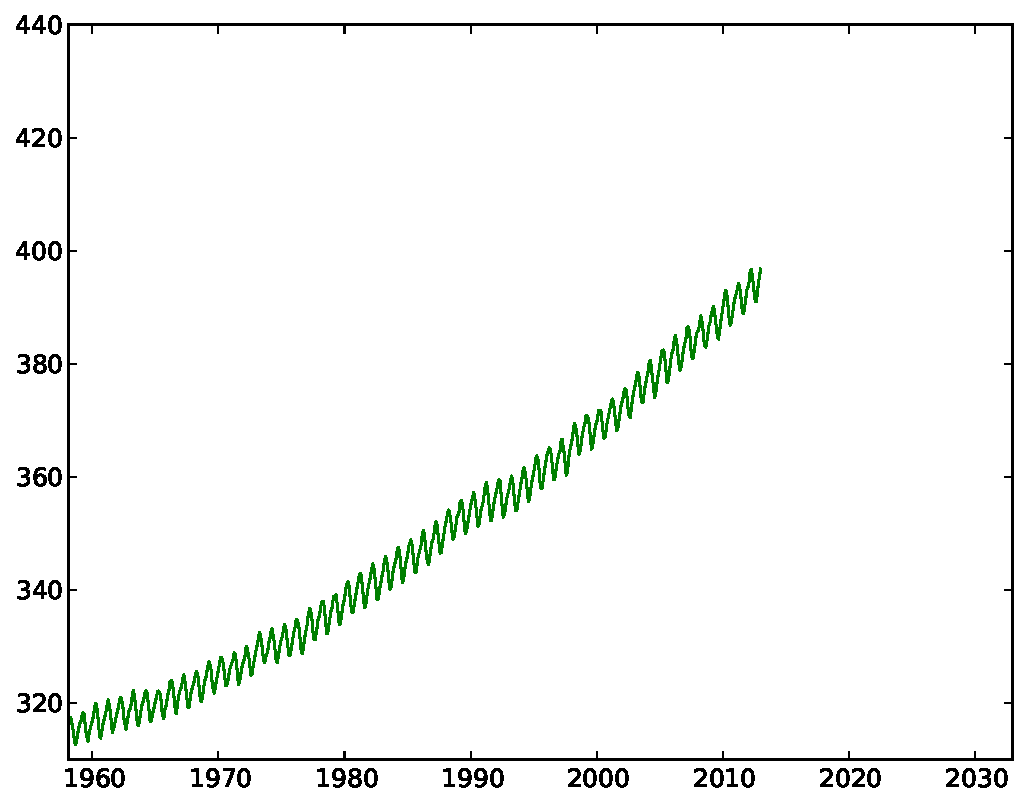
\includegraphics[height=4.5cm]{figures/python/CO2-data}
\end{center}
Let's try to predict the concentration for the next 20 years.
\end{example}
\end{frame}

%%%%%%%%%%%%%%%%%%%%%%%%%%%%%%%%%%%%%%%%%%%%%%%%%%%%%%
\begin{frame}{Sum of kernels over the same space }
We first consider a squared-exponential kernel: 
$$ \displaystyle k(x,y) = \sigma^2\exp \left(-\frac{(x-y)^2}{\theta^2} \right)$$
\begin{center}
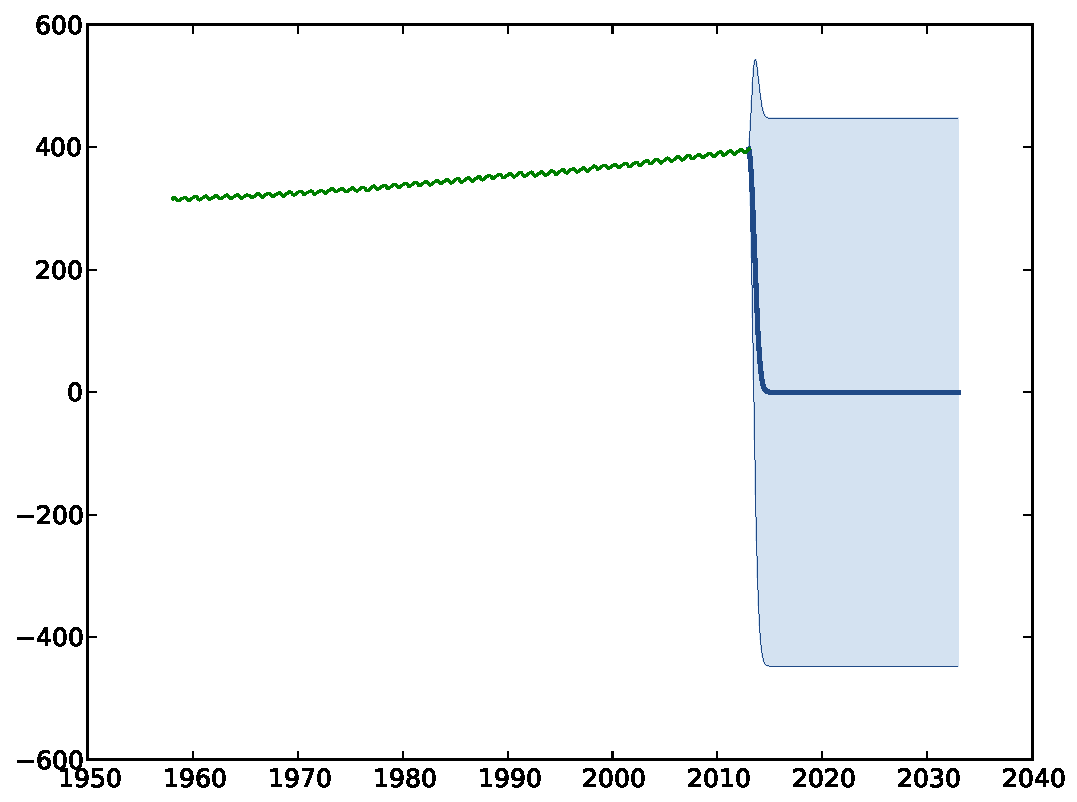
\includegraphics[width=.48\textwidth]{figures/python/CO2-rbfa} \hfill 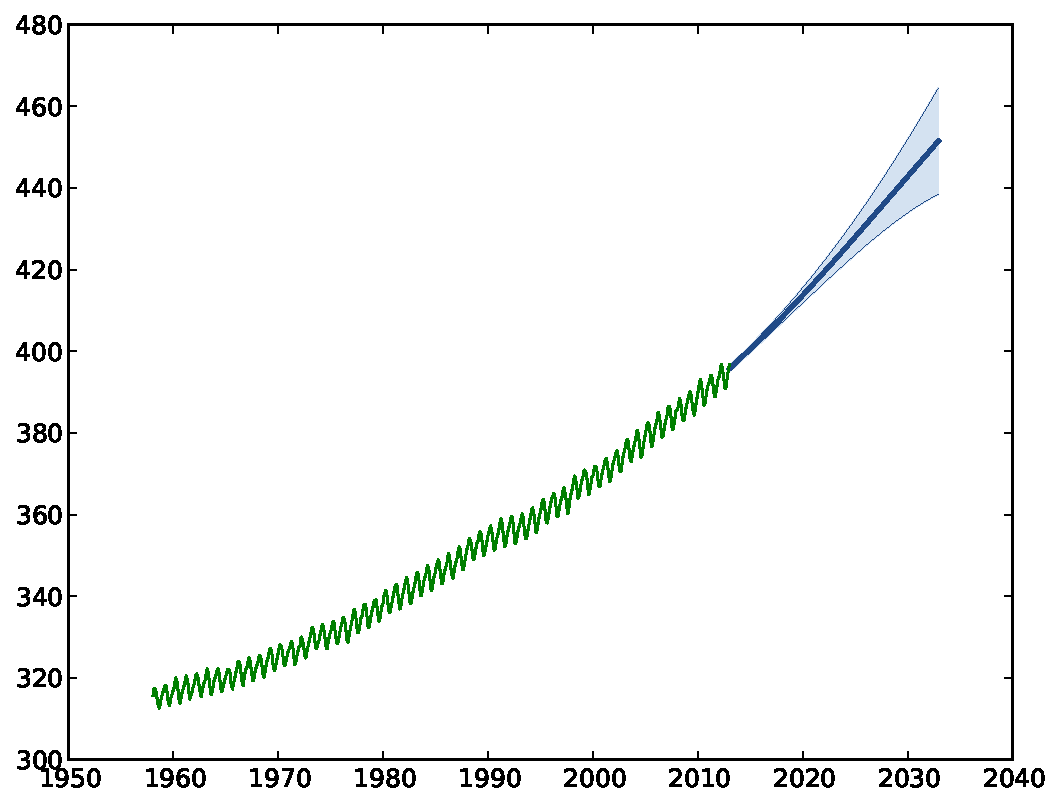
\includegraphics[width=.48\textwidth]{figures/python/CO2-rbfb}
\end{center}
\vspace{5mm}
\begin{block}{}
\centering
\alert{The results are terrible!}
\end{block}
\end{frame}

%%%%%%%%%%%%%%%%%%%%%%%%%%%%%%%%%%%%%%%%%%%%%%%%%%%%%%
\begin{frame}{Sum of kernels over the same space }
What happen if we sum both kernels?
\begin{equation*}
k(x,y) = k_{rbf1}(x,y) + k_{rbf2}(x,y)
\end{equation*} 
\pause
\begin{center}
\vspace{-8mm} 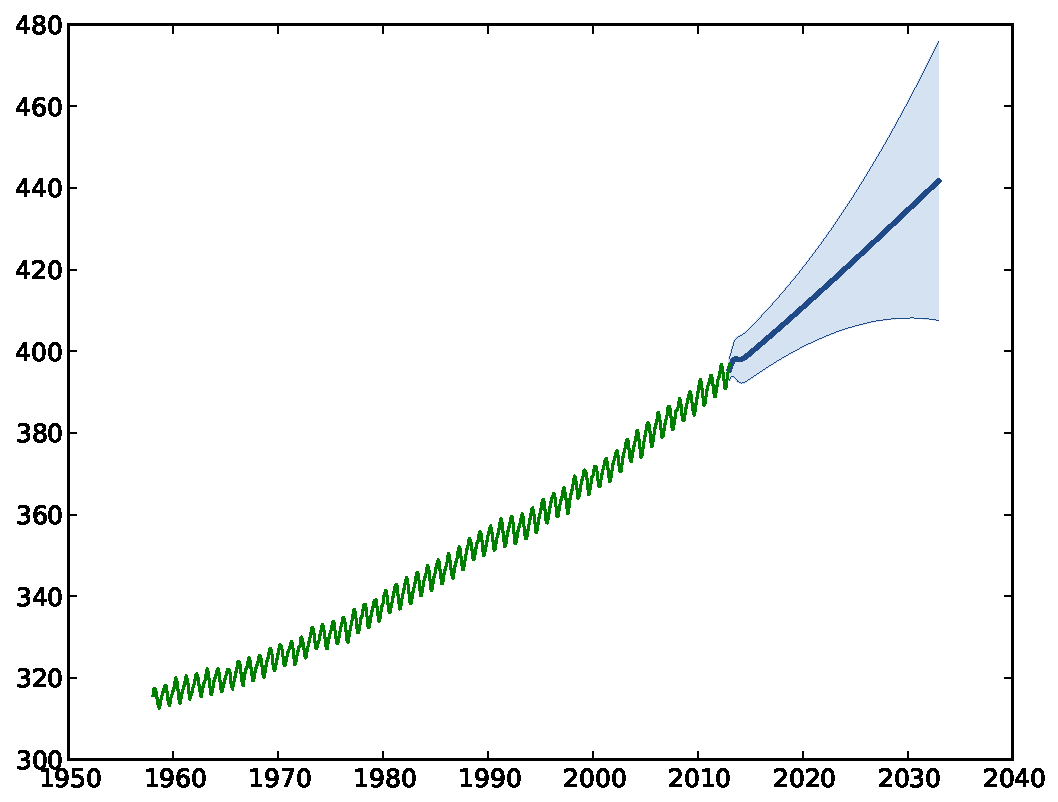
\includegraphics[height=4.5cm]{figures/python/CO2-rbfab}
\end{center}
%\vspace{1mm}
\begin{block}{}
\centering
\alert{The model is drastically improved!}
\end{block}
\end{frame}

%%%%%%%%%%%%%%%%%%%%%%%%%%%%%%%%%%%%%%%%%%%%%%%%%%%%%%
\begin{frame}{Sum of kernels over the same space }
We can try the following kernel:
\begin{equation*}
k(x,y) = \sigma_0^2  x^2 y^2 + k_{rbf1}(x,y) + k_{rbf2}(x,y) + k_{per}(x,y)
\end{equation*}
\pause
\begin{center}
\vspace{-8mm}  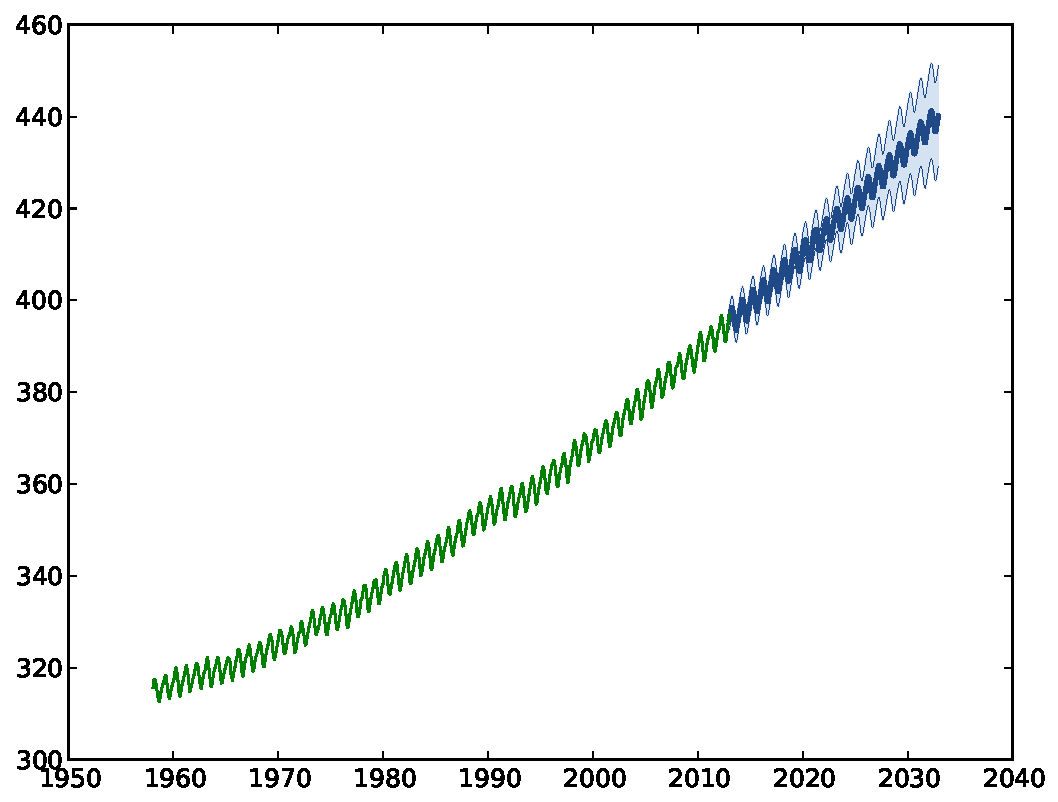
\includegraphics[height=4.5cm]{figures/python/CO2-rbfabpq}
\end{center}
\begin{block}{}
\centering
\alert{Once again, the model is significantly improved.}
\end{block}
\end{frame}


%%%%%%%%%%%%%%%%%%%%%%%%%%%%%%%%%%%%%%%%%%%%%%%%%%%%%%
\begin{frame}{Sum of kernels over tensor space}
\begin{block}{Property}
\begin{equation*}
k(\textbf{x},\textbf{y}) = k_1(x_1,y_1) +  k_2(x_2,y_2)
\end{equation*} is a valid covariance structure.\\
\begin{columns}[c]
\begin{column}{3cm}
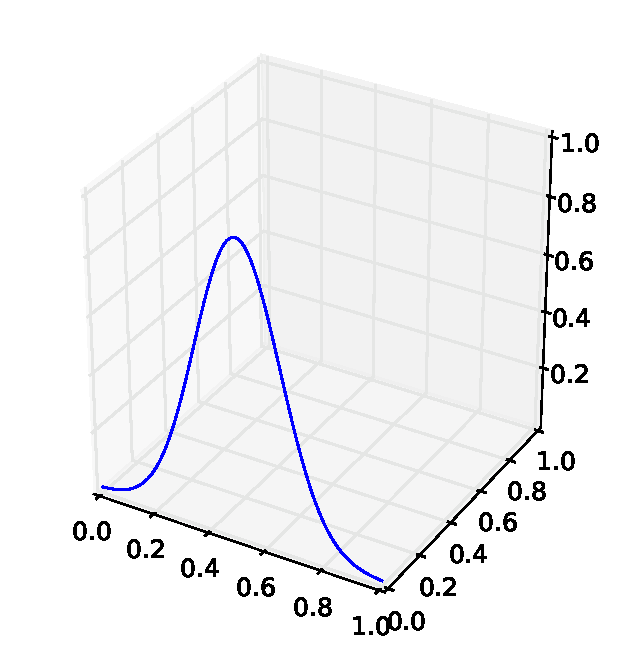
\includegraphics[width=3cm]{figures/python/newfromold-sum2-k1}
\end{column}
\begin{column}{2mm}
$+$
\end{column}
\begin{column}{3cm}
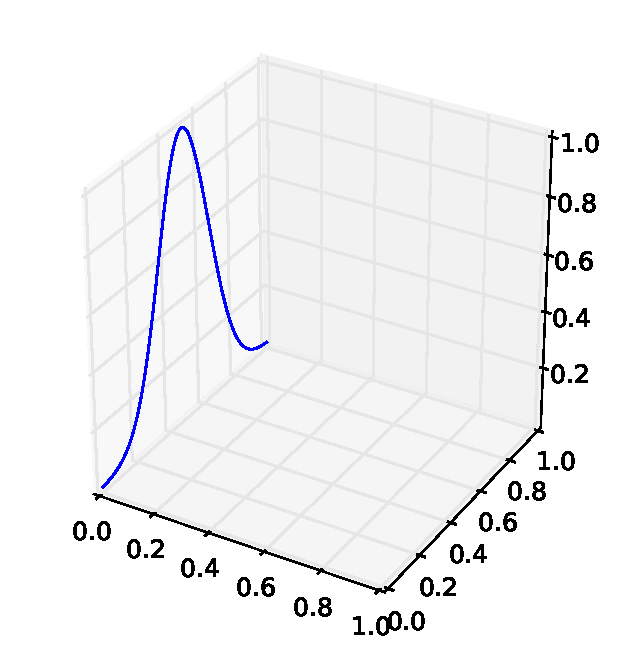
\includegraphics[width=3cm]{figures/python/newfromold-sum2-k2}
\end{column}
\begin{column}{2mm}
$=$
\end{column}
\begin{column}{3cm}
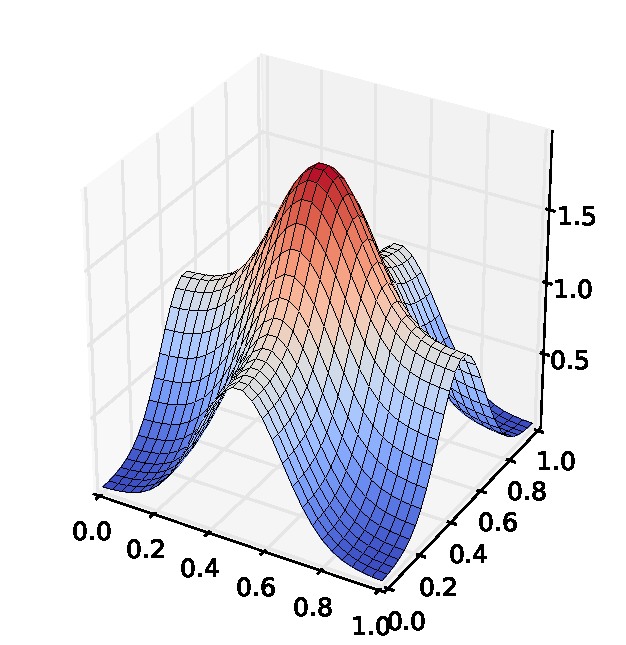
\includegraphics[width=3cm]{figures/python/newfromold-sum2-k12}
\end{column}
\end{columns}
\vspace{4mm}
\end{block} \ \\
\structure{Remark:}
\begin{itemize}
 \item From a GP point of view, $k$ is the kernel of $Z(\textbf{x}) = Z_1(x_1) + Z_2(x_2)$
\end{itemize}
\end{frame}

%%%%%%%%%%%%%%%%%%%%%%%%%%%%%%%%%%%%%%%%%%%%%%%%%%%%%%
\begin{frame}{Sum of kernels over tensor space}
We can have a look at a few sample paths from $Z$:
\begin{center}
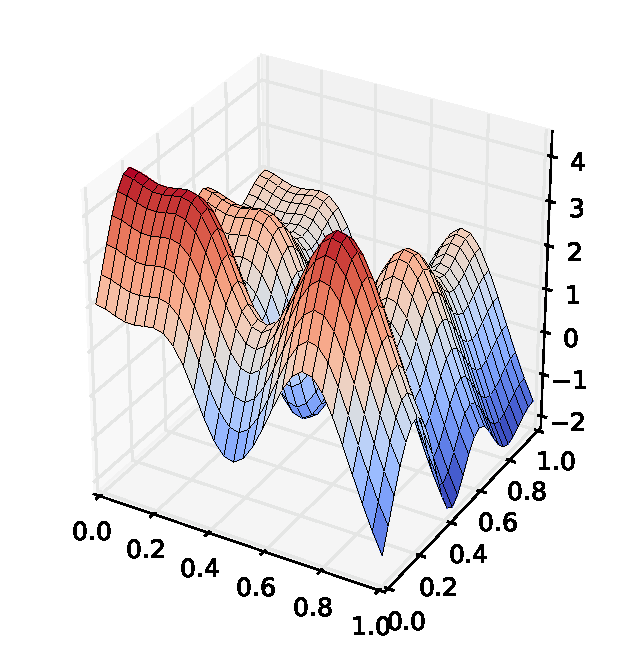
\includegraphics[width=3.5cm]{figures/python/newfromold-sum2-traj124} 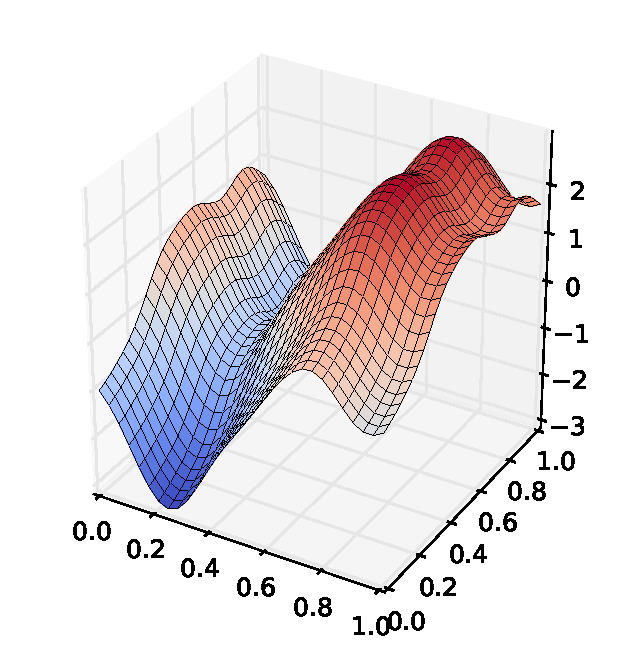
\includegraphics[width=3.5cm]{figures/python/newfromold-sum2-traj121} 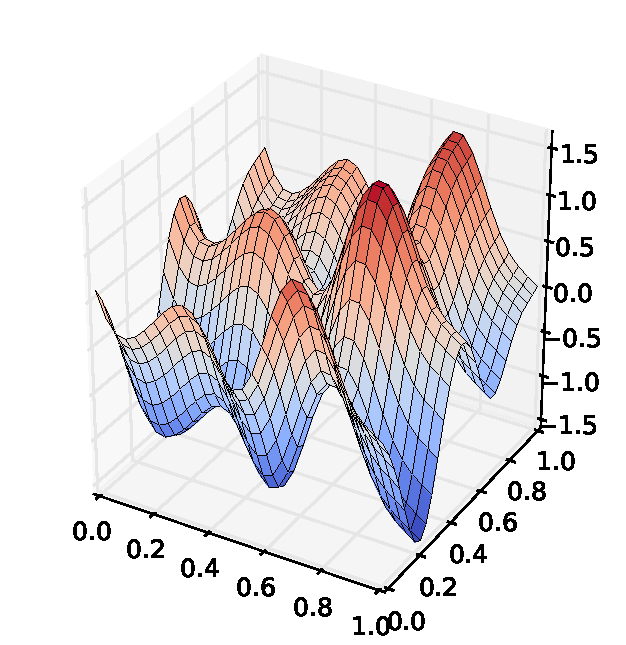
\includegraphics[width=3.5cm]{figures/python/newfromold-sum2-traj123} % 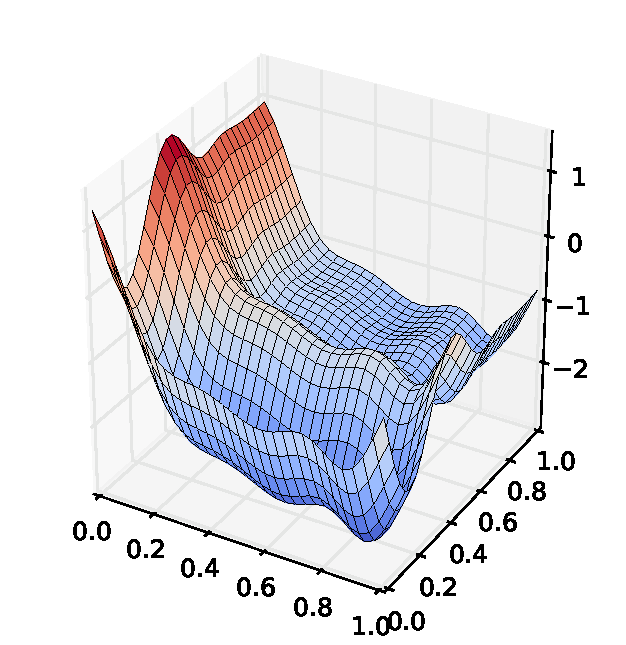
\includegraphics[width=3.5cm]{Figures/newfromold-sum2-traj122} 
\end{center}
\qquad \alert{$\Rightarrow$ They are additive (up to a modification)}\\ \ \\
Tensor Additive kernels are very useful for
\begin{itemize}
  \item Approximating additive functions
  \item Building models over high dimensional inputs spaces
\end{itemize}
\end{frame}

%%%%%%%%%%%%%%%%%%%%%%%%%%%%%%%%%%%%%%%%%%%%%%%%%%%%%%
\begin{frame}{Sum of kernels over tensor space}
We consider the test function $f(x) = \sin( 4 \pi x_1) + \cos( 4 \pi x_2) + 2 x_2$ and a set of 20 observation in $[0,1]^2$ \\ \vspace{5mm}
\begin{columns}[c]
\begin{column}{5cm}
\textbf{Test function}
\begin{center}
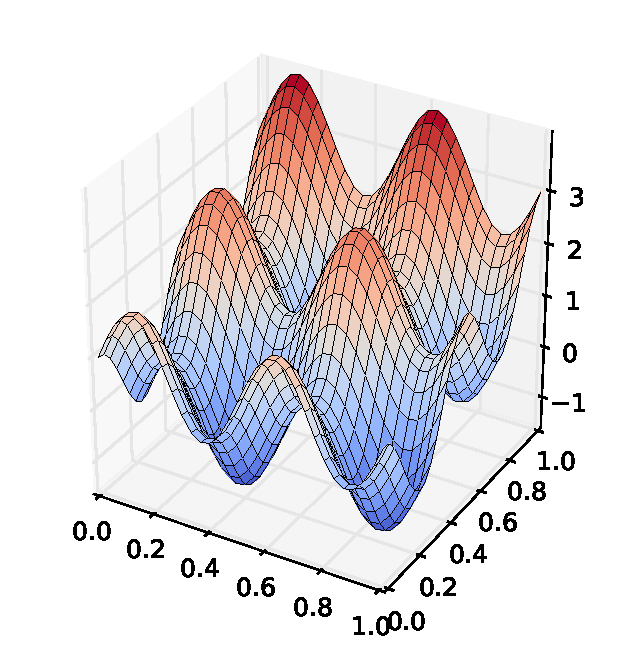
\includegraphics[height=4cm]{figures/python/newfromold-productvssum2-predt}
\end{center}
\end{column}
\begin{column}{5cm}
\textbf{Observations}
\begin{center}
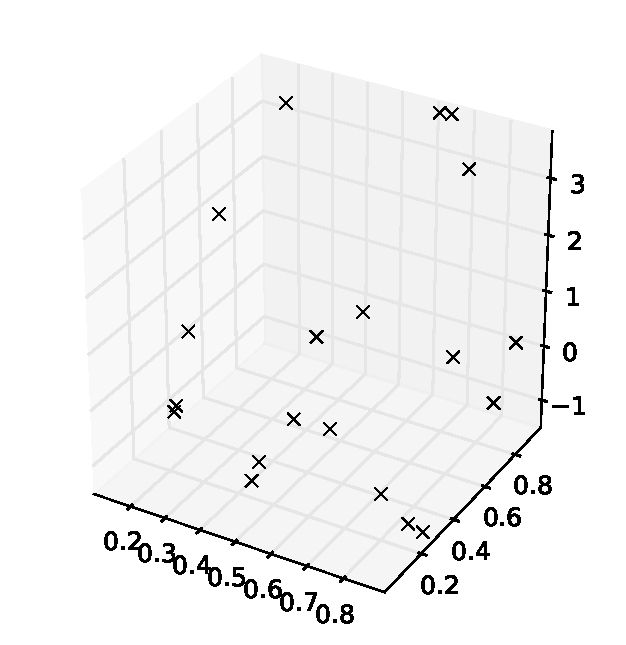
\includegraphics[height=4cm]{figures/python/newfromold-productvssum2-preddoe}
\end{center}
\end{column}
\end{columns} 
\vspace{5mm}
\
\end{frame}

%%%%%%%%%%%%%%%%%%%%%%%%%%%%%%%%%%%%%%%%%%%%%%%%%%%%%%
\begin{frame}{Sum of kernels over tensor space}
We obtain the following models:\\ \vspace{5mm}
\begin{columns}[c]
\begin{column}{5cm}
\textbf{Gaussian kernel}
\begin{center}
Mean predictor
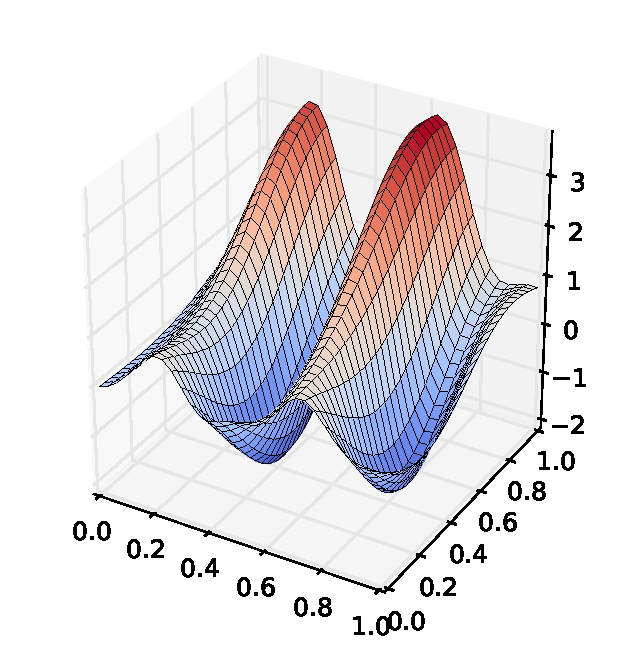
\includegraphics[height=4cm]{figures/python/newfromold-productvssum2-predp}\\
RMSE is 1.06
\end{center}
\end{column}
\begin{column}{5cm}
\textbf{Additive Gaussian kernel}
\begin{center}
Mean predictor
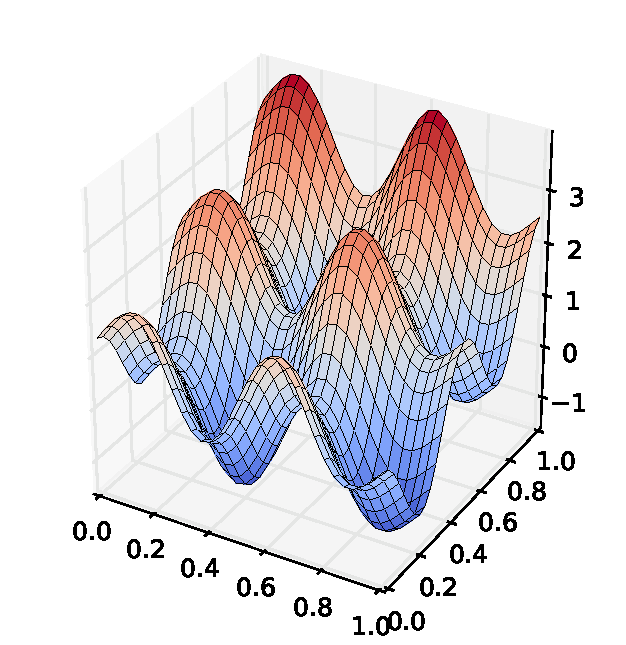
\includegraphics[height=4cm]{figures/python/newfromold-productvssum2-preda}\\
RMSE is 0.12
\end{center}
\end{column}
\end{columns} 
\end{frame}

%%%%%%%%%%%%%%%%%%%%%%%%%%%%%%%%%%%%%%%%%%%%%%%%%%%%%%
\begin{frame}{Sum of kernels over tensor space}
\begin{block}{Remarks}%[(continuation)]
\begin{itemize}
\item It is straightforward to show that the mean predictor is additive
 \small
 \begin{equation*}
 \begin{split}
  m(\mathbf{x}) & = (k_1(x,X) + k_2(x,X)) (k(X,X))^{-1} F \\
  &  = \underbrace{k_1(x_1,X_1) (k(X,X))^{-1} F}_{m_1(x_1)}  + \underbrace{k_2(x_2,X_2) (k(X,X))^{-1} F}_{m_2(x_2)} 
 \end{split}
 \end{equation*}
\alert{ $\Rightarrow$ The model shares the prior behaviour.}
 \normalsize
\vspace{5mm}
 \item The sub-models can be interpreted as GP regression models with observation noise: 
  \begin{equation*}
  m_1(x_1) = \E{\ Z_1(x_1)\ |\  Z_1(X_1)+Z_2(X_2) \shorteq F\ }
 \end{equation*}
\end{itemize}
\end{block}
\end{frame}

%%%%%%%%%%%%%%%%%%%%%%%%%%%%%%%%%%%%%%%%%%%%%%%%%%%%%%
\begin{frame}{Sum of kernels over tensor space}
\begin{block}{Remark}%[(continuation)]
\begin{itemize}
\item The prediction variance has interesting features
\begin{columns}[c]
\begin{column}{5cm}
\begin{center}
pred. var. with kernel product
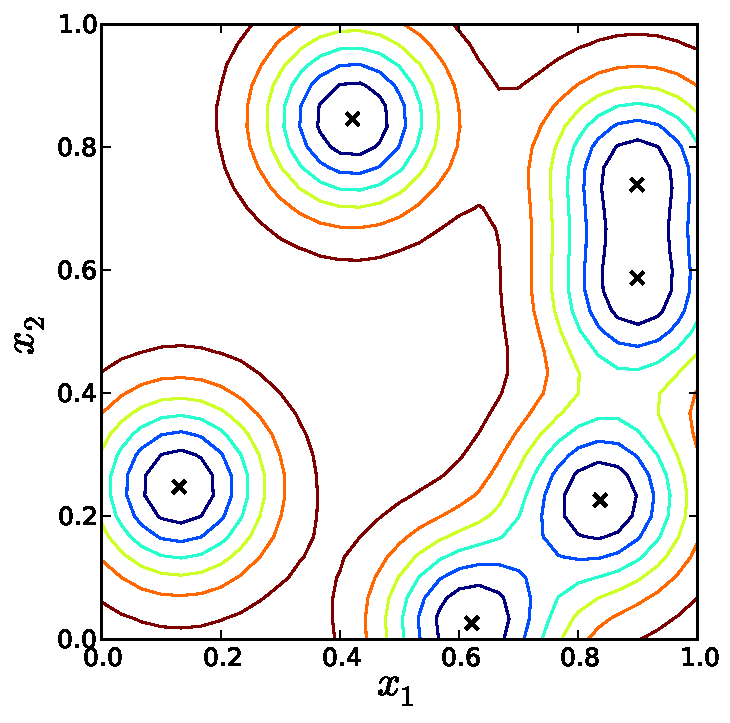
\includegraphics[height=4cm]{figures/python/kernelmodels-predvarprod}
\end{center}
\end{column}
\begin{column}{5cm}
\begin{center}
pred. var. with kernel sum
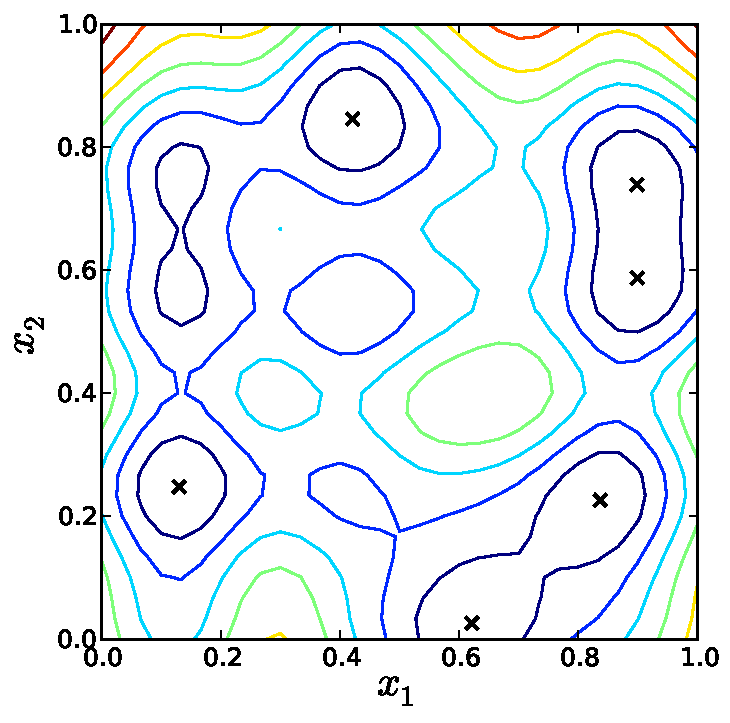
\includegraphics[height=4cm]{figures/python/kernelmodels-predvar}
\end{center}
\end{column}
\end{columns}
\end{itemize} 
\end{block}
\end{frame}

%%%%%%%%%%%%%%%%%%%%%%%%%%%%%%%%%%%%%%%%%%%%%%%%%%%%%%
\begin{frame}{Sum of kernels over tensor space}
This property can be used to construct a design of experiment that covers the space with only $cst \times d$ points.
\begin{center}
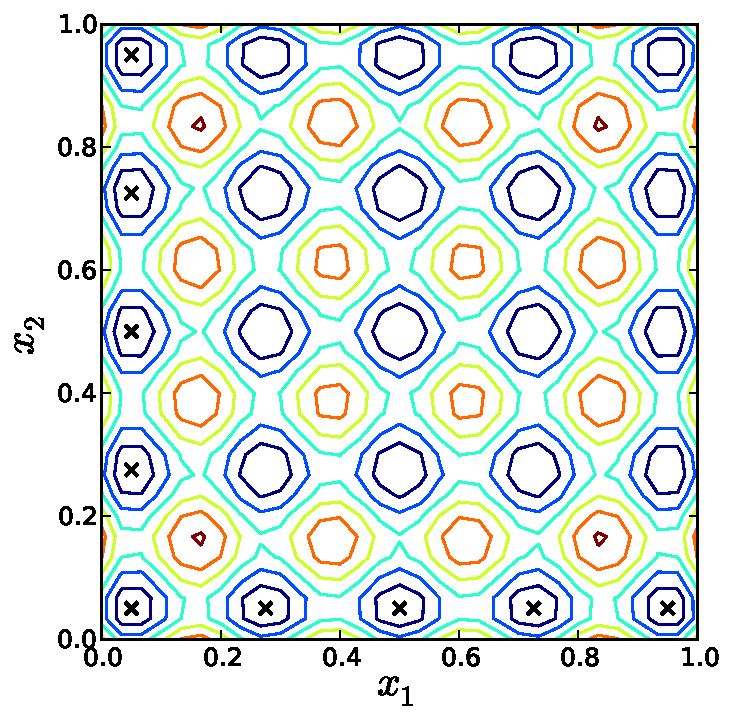
\includegraphics[height=5cm]{figures/python/kernelmodels-predaxe}\\
Prediction variance
\end{center}
\vfill
\end{frame}


%%%%%%%%%%%%%%%%%%%%%%%%%%%%%%%%%%%%%%%%%%%%%%%%%%%%%%
%%%%%%%%%%%%%%%%%%%%%%%%%%%%%%%%%%%%%%%%%%%%%%%%%%%%%%
%\subsection{Product of kernels}

%%%%%%%%%%%%%%%%%%%%%%%%%%%%%%%%%%%%%%%%%%%%%%%%%%%%%%
\begin{frame}{Product over the same space}
\begin{block}{Property}
\begin{equation*}
k(x,y) = k_1(x,y) \times  k_2(x,y)
\end{equation*}
is valid covariance structure.
\end{block}
%\vspace{10mm}
\begin{example}
We consider the product of a squared exponential with a cosine:
\begin{columns}[c]
\begin{column}{3cm}
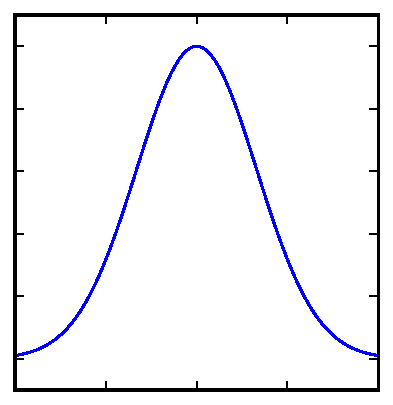
\includegraphics[width=3cm]{figures/python/newfromold-pa.pdf}
\end{column}
\begin{column}{2mm}
$\times$
\end{column}
\begin{column}{3cm}
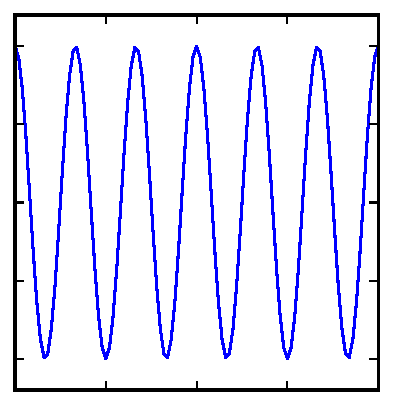
\includegraphics[width=3cm]{figures/python/newfromold-pb.pdf}
\end{column}
\begin{column}{2mm}
$=$
\end{column}
\begin{column}{3cm}
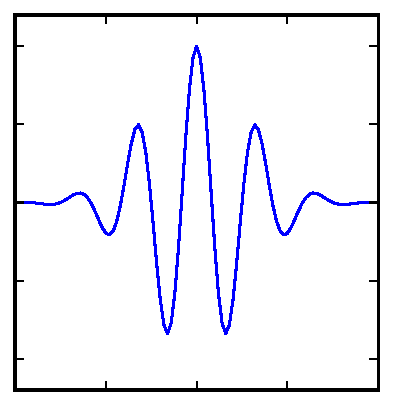
\includegraphics[width=3cm]{figures/python/newfromold-pab1.pdf}
\end{column}
\end{columns}
\vspace{5mm}
\end{example}
\end{frame}

%%%%%%%%%%%%%%%%%%%%%%%%%%%%%%%%%%%%%%%%%%%%%%%%%%%%%%
\begin{frame}{Product over the tensor space}
\begin{block}{Property}
\begin{equation*}
k(\textbf{x},\textbf{y}) = k_1(x_1,y_1) \times k_2(x_2,y_2)
\end{equation*}
is valid covariance structure.
\end{block}
%\vspace{10mm}
\begin{example}
We multiply 2 squared exponential kernel
\begin{columns}[c]
\begin{column}{3cm}
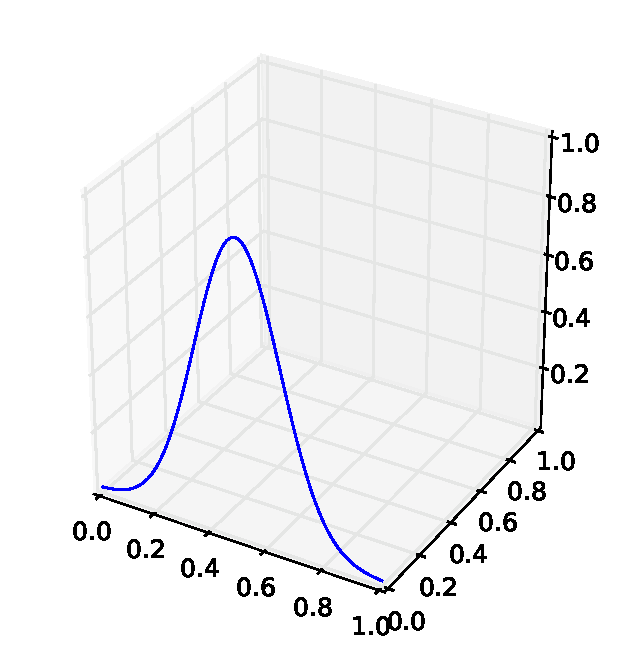
\includegraphics[width=3cm]{figures/python/newfromold-sum2-k1}
\end{column}
\begin{column}{2mm}
$\times $
\end{column}
\begin{column}{3cm}
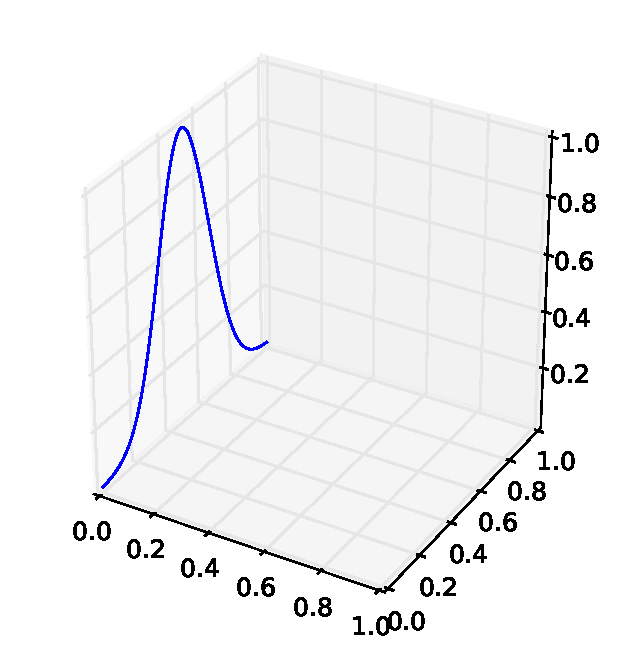
\includegraphics[width=3cm]{figures/python/newfromold-sum2-k2}
\end{column}
\begin{column}{2mm}
$=$
\end{column}
\begin{column}{3cm}
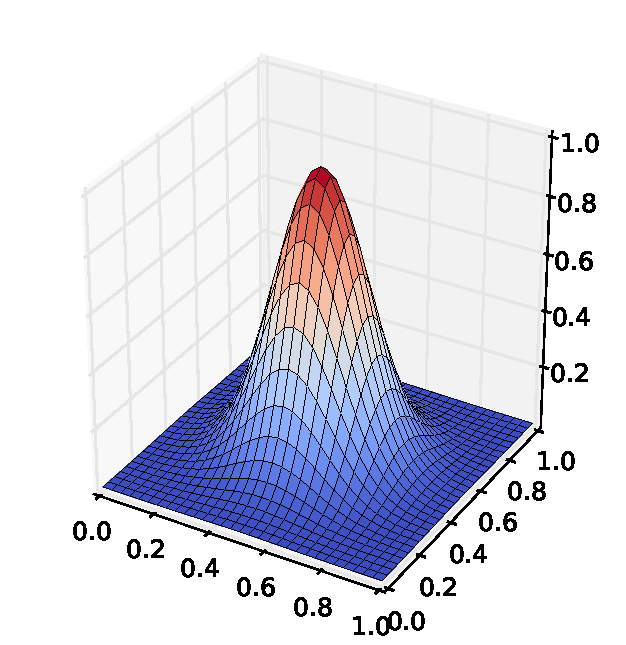
\includegraphics[width=3cm]{figures/python/newfromold-prod2-k12}
\end{column}
\end{columns}
\vspace{5mm}
\structure{\textbf{Question:}} What kernel do we end up with?
\end{example}
\end{frame}


%%%%%%%%%%%%%%%%%%%%%%%%%%%%%%%%%%%%%%%%%%%%%%%%%%%%%%
%%%%%%%%%%%%%%%%%%%%%%%%%%%%%%%%%%%%%%%%%%%%%%%%%%%%%%
%\subsection{Composition with a function}

%%%%%%%%%%%%%%%%%%%%%%%%%%%%%%%%%%%%%%%%%%%%%%%%%%%%%%
\begin{frame}{Composition with a function}
\begin{block}{Property}
Let $k_1$ be a kernel over $D_1 \times D_1$ and $f$ be an arbitrary function $D \rightarrow D_1$, then
\begin{equation*}
k(x,y) = k_1(f(x),f(y))
\end{equation*}
is a kernel over $D \times D $.\\
\small
\textbf{proof}\\
\begin{equation*}
\sum \sum a_i  a_j k(x_i,x_j) = \sum \sum a_i a_j k_1(\underbrace{f(x_i)}_{y_i},\underbrace{f(x_j)}_{y_j}) \geq 0 
\end{equation*}
\end{block}
\vspace{5mm}
\structure{Remarks:}
\begin{itemize}
\item $k$ corresponds to the covariance of $Z(x) = Z_1(f(x))$
\item This can be seen as a (nonlinear) rescaling of the input space
\end{itemize}
\end{frame}

%%%%%%%%%%%%%%%%%%%%%%%%%%%%%%%%%%%%%%%%%%%%%%%%%%%%%%
\begin{frame}{}
\begin{example}
We consider $f(x) = \frac1x$ and a Mat\'ern 3/2 kernel $k_1(x,y) = (1 + |x-y|) e^{-|x-y|}$.\\ \vspace{5mm}
\textbf{We obtain:}
\begin{columns}[c]
\begin{column}{5cm}
\begin{center}
Kernel
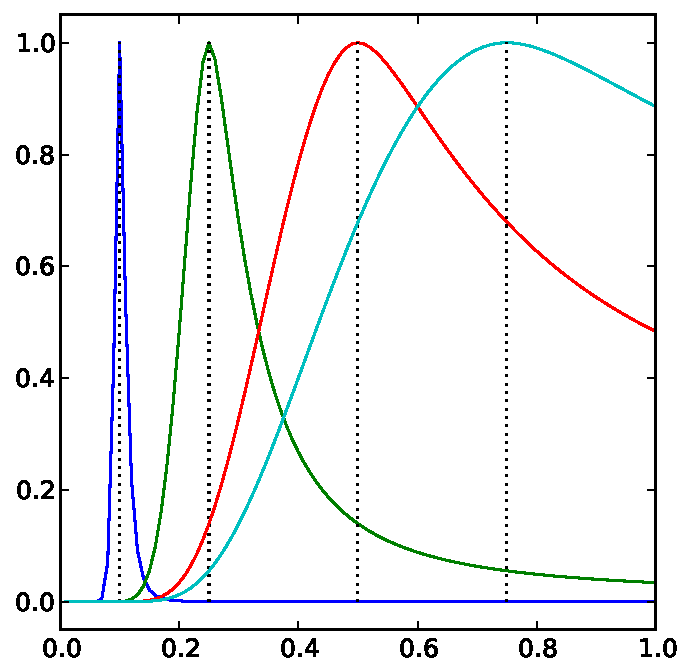
\includegraphics[width=4cm]{figures/python/newfromold-compfunc-k}
\end{center}
\end{column}
\begin{column}{5cm}
\begin{center}
Sample paths
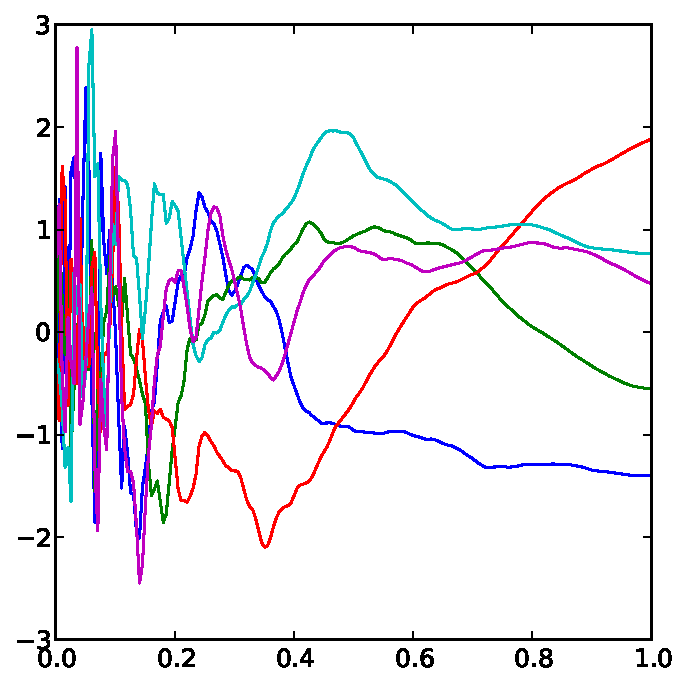
\includegraphics[width=4cm]{figures/python/newfromold-compfunc-traj}
\end{center}
\end{column}
\end{columns}
\end{example}
\end{frame}

%%%%%%%%%%%%%%%%%%%%%%%%%%%%%%%%%%%%%%%%%%%%%%%%%%%%%%
\begin{frame}{}
\structure{All these transformations can be combined!}
\begin{example}
$k(x,y) = f(x)f(y)k_1(x,y)$ is a valid kernel.\\
\vspace{0.5cm}
This can be illustrated with $f(x) = \frac1x$ and $k_1(x,y) = (1 + |x-y|) e^{-|x-y|}$:\\ 
\begin{columns}[c]
\begin{column}{5cm}
\begin{center}
Kernel
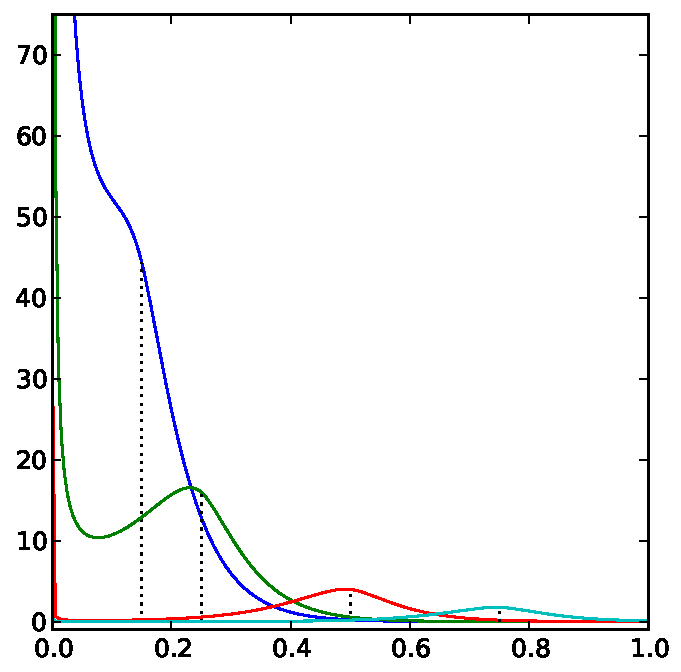
\includegraphics[width=4cm]{figures/python/newfromold-prodfunc-k}
\end{center}
\end{column}
\begin{column}{5cm}
\begin{center}
Sample paths
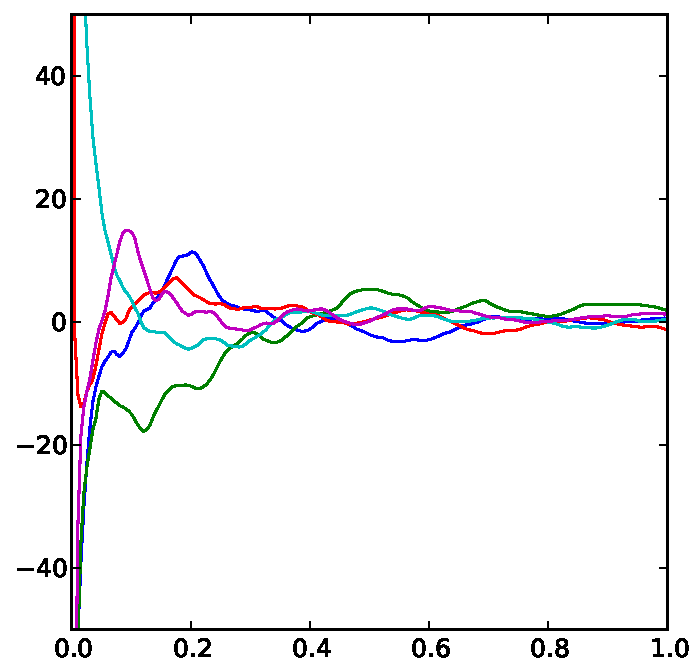
\includegraphics[width=4cm]{figures/python/newfromold-prodfunc-traj}
\end{center}
\end{column}
\end{columns}
\end{example}
\end{frame}

%%%%%%%%%%%%%%%%%%%%%%%%%%%%%%%%%%%%%%%%%%%%%%%%%%%%%%%%%%%%%%%%%%%%%%%%%%%%%%%%%%%%
%%%%%%%%%%%%%%%%%%%%%%%%%%%%%%%%%%%%%%%%%%%%%%%%%%%%%%%%%%%%%%%%%%%%%%%%%%%%%%%%%%%%
\section[linear operator]{Effect of a linear operator}
\subsection{}

%%%%%%%%%%%%%%%%%%%%%%%%%%%%%%%%%%%%%%%%%%%%%%%%%%%%%%
\begin{frame}{Effect of a linear operator}
\begin{block}{Property}
Let $L$ be a linear operator that can be applied to samples of a process $Z$ {\tiny(such that [...])}. Then
    \begin{equation*}
        k(x,y) = L_x(L_y(k(x,y)))
    \end{equation*}
\end{block}
\begin{example}
  We want to approximate a function $[0,1] \rightarrow \mathds{R}$ that is symmetric with respect to $0.5$.
We will consider 2 linear operators:
\begin{equation*}
 L_1 : f(x) \rightarrow 
\left\{ 
\begin{aligned}
 f(x) \text{\qquad}  & x < 0.5 \\
 f(1-x) \text{\qquad}   & x \geq 0.5 
\end{aligned}
\right.
\end{equation*}
$$ L_2 : f(x) \rightarrow \frac{f(x) + f(1-x)}{2}.$$
\end{example}
\end{frame}

%%%%%%%%%%%%%%%%%%%%%%%%%%%%%%%%%%%%%%%%%%%%%%%%%%%%%%
\begin{frame}{Effect of a linear operator: example [Ginsbourger 2013]}
Examples of associated sample paths are 

\begin{columns}[c]
\begin{column}{5cm}
\begin{center}
 $k_1 = L_1(L_1(k))$
\end{center}
 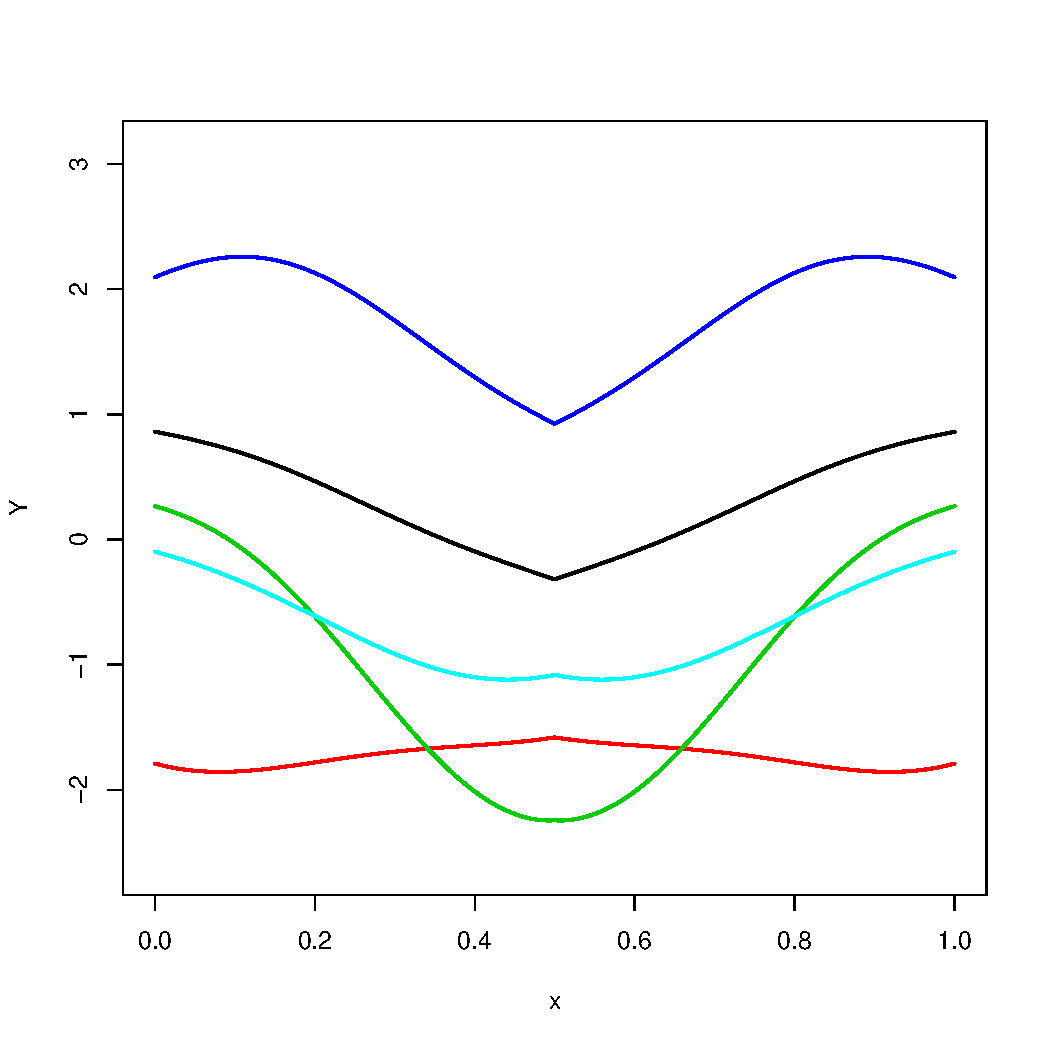
\includegraphics[height=5cm]{figures/p2-sym1}
\end{column}
\begin{column}{5cm}
\begin{center}
 $k_2= L_2(L_2(k))$
\end{center}
 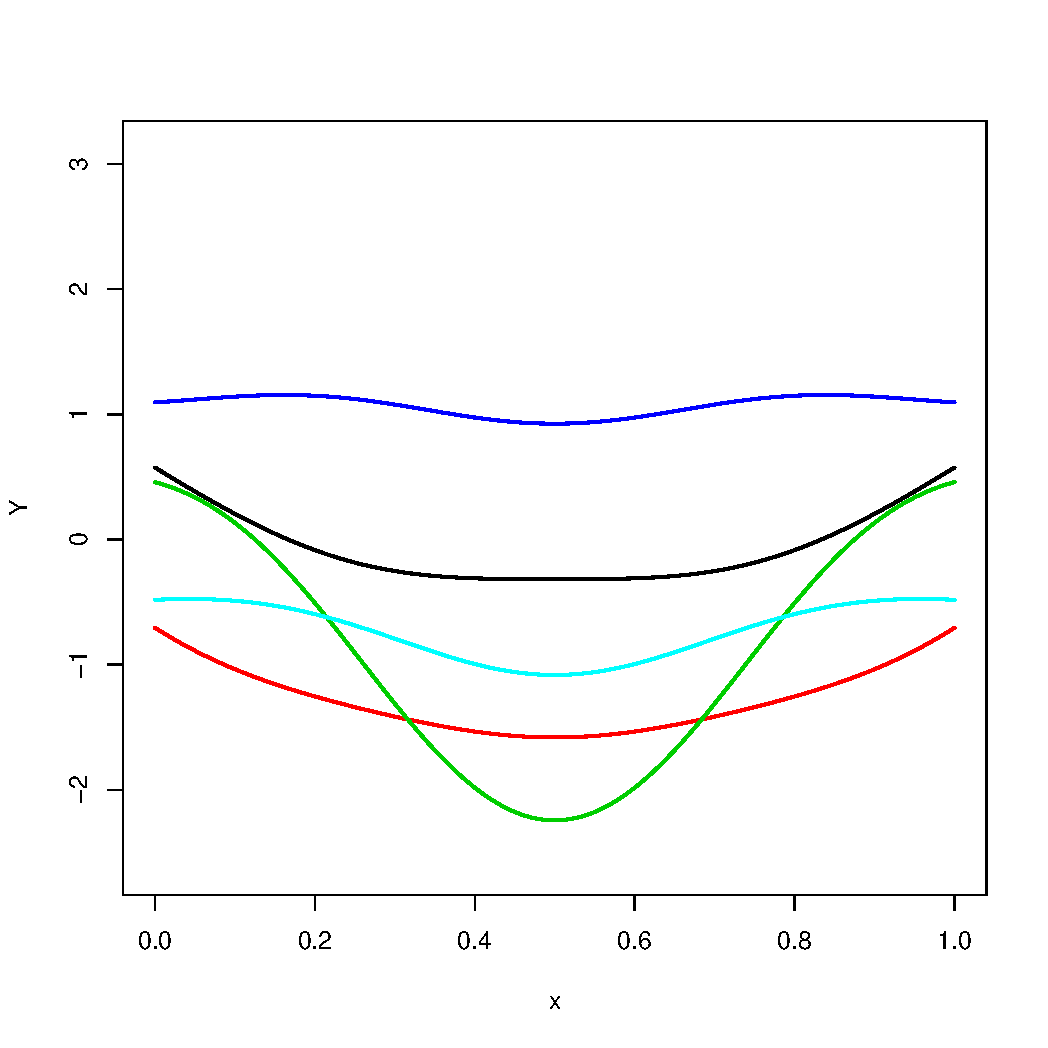
\includegraphics[height=5cm]{figures/p2-sym2}
\end{column}
\end{columns}
The differentiability is not always respected!
\end{frame}

%%%%%%%%%%%%%%%%%%%%%%%%%%%%%%%%%%%%%%%%%%%%%%%%%%%%%%
\begin{frame}{Effect of a linear operator}
These linear operators are projections onto a space of symmetric functions:
\begin{center}
\vspace{0.5cm}
 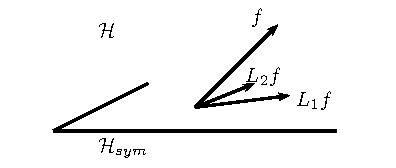
\includegraphics[height=2cm]{figures/proj-sym}
\vspace{0.5cm}
\end{center}
What about the optimal projection?\\
\vspace{0.5cm}
\alert{$\Rightarrow$ This can be difficult... but it raises interesting questions!}
\end{frame}

%%%%%%%%%%%%%%%%%%%%%%%%%%%%%%%%%%%%%%%%%%%%%%%%%%%%%%
%%%%%%%%%%%%%%%%%%%%%%%%%%%%%%%%%%%%%%%%%%%%%%%%%%%%%%
\section{Conclusion}
\subsection{}


%%%%%%%%%%%%%%%%%%%%%%%%%%%%%%%%%%%%%%%%%%%%%%%%%%%%%%
\begin{frame}{}
We have seen that \vspace{2mm}
\begin{itemize}
 \item Kriging model do not necessarily interpolate, but they can if we want them to!
 \item If we have information about a trend, it is possible to incorporate it in models.
 \item Kernels encode the prior belief on the function to approximate.
 \begin{itemize}
 	\item They should be chosen accordingly
 \end{itemize}
 \item It is sometimes possible to design kernels tailored to the problem at hand.
\end{itemize}
\end{frame}



%%%%%%%%%%%%%%%%%%%%%%%%%%%%%%%%%%%%%%%%%%%%%%%%%%%%%%%%%%%%%%%%%%%%%%%%%%%%%%%
%%%%%%%%%%%%%%%%%%%%%%%%%%%%%%%%%%%%%%%%%%%%%%%%%%%%%%%%%%%%%%%%%%%%%%%%%%%%%%%
%%%%%%%%%%%%%%%%%%%%%%%%%%%%%%%%%%%%%%%%%%%%%%%%%%%%%%%%%%%%%%%%%%%%%%%%%%%%%%%
%%%%%%%%%%%%%%%%%%%%%%%%%%%%%%%%%%%%%%%%%%%%%%%%%%%%%%%%%%%%%%%%%%%%%%%%%%%%%%%
\end{document}



\structure{}

\begin{center}
  \begin{tabular}{|c|cc|}

  \end{tabular}
\end{center}

###
%%%%%%%%%%%%%%%%%%%%%%%%%%%%%%%%%%%%%%%%%%%%%%%%%%%%%%
\begin{frame}{}

\end{frame}

###
\begin{block}{}

\end{block}

###
\begin{center}
\includegraphics[height=5cm]{figures/}
\end{center}

###
\begin{columns}[c]
\column{5cm}

\column{5cm}

\end{columns}
